\chapter{RESULTADOS E DISCUSSÃO}\label{cap:resultados}

Neste capítulo são apresentados e discutidos os resultados obtidos ao longo do desenvolvimento experimental e computacional da plataforma proposta. Inicialmente, expõem-se os resultados dos ensaios de bancada voltados à calibração e à caracterização estocástica dos sensores embarcados, cujas variâncias medidas fundamentam a parametrização do Filtro de Kalman. Na sequência, apresentam-se os resultados das simulações numéricas em malha fechada conduzidas no ambiente MATLAB/Simulink, comparando o desempenho do controlador LQG aplicado ao modelo linearizado e à planta dinâmica não linear do quadricóptero. Por fim, apresentam-se o ensaio de voo real, os ensaios de comunicação entre o Raspberry Pi e o STM32 e os resultados do planejamento de rotas.

% =============================================================
\section{CARACTERIZAÇÃO EXPERIMENTAL E CALIBRAÇÃO DOS SENSORES}\label{sec:res_sensores}

Conforme estabelecido na metodologia (Seção~\ref{subsec:modelagem_projeto_controle}), a implementação prática do Filtro de Kalman exige o conhecimento prévio da matriz de covariância do ruído de medição $\mathbf{R}_v$, evitando que a sintonia do estimador dependa exclusivamente de ajustes empíricos. Para determinar as variâncias reais ($\sigma_v^2$) de cada canal sensorial, realizaram-se ensaios estáticos de bancada com a plataforma imobilizada sobre uma superfície nivelada, sem acionamento dos propulsores.

\subsection{Análise de ruído e desempenho temporal da IMU BNO08X}\label{subsec:res_bno08x}

Durante o ensaio estático da unidade de medição inercial BNO08X, foram coletadas $N = 1092$ amostras consecutivas, registradas a 10~Hz pelo \textit{log} USB, com os \textit{reports} da IMU configurados a uma taxa nominal de 100~Hz via barramento I$^2$C2 a 400~kHz. A Figura~\ref{fig:ruido_bno08x} apresenta o comportamento temporal das leituras dos ângulos de Euler ($\phi, \theta, \psi$) e das velocidades angulares ($p, q, r$). A Figura~\ref{fig:bancada_bno08x} mostra a montagem em protoboard usada nesse ensaio, com a IMU ligada à placa STM32F411.

\begin{figure}[H]
    \centering
    \caption{Montagem em protoboard para o ensaio de bancada da IMU BNO08X com o STM32F411.}
    \label{fig:bancada_bno08x}
    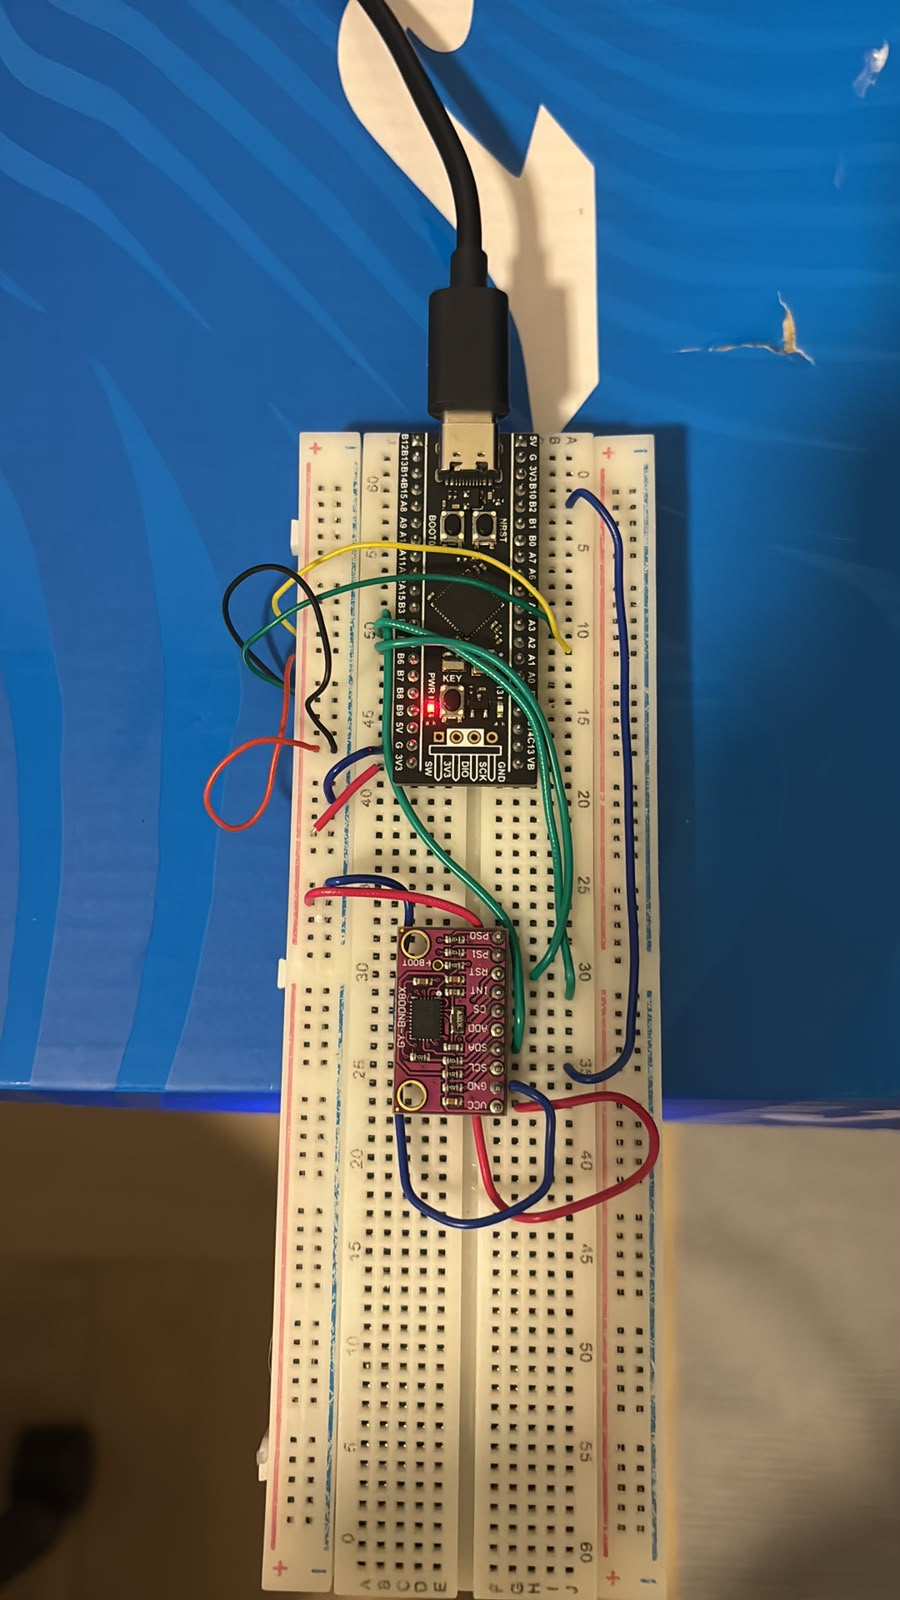
\includegraphics[width=0.4\textwidth]{images/testes/bno-bancada.png}
    \par\vspace{0.2cm}
    \footnotesize Fonte: elaborado pelos autores (2026).
\end{figure}

\begin{figure}[H]
    \centering
    \caption{Leituras estáticas e distribuição de ruído dos canais da IMU BNO08X.}
    \label{fig:ruido_bno08x}
    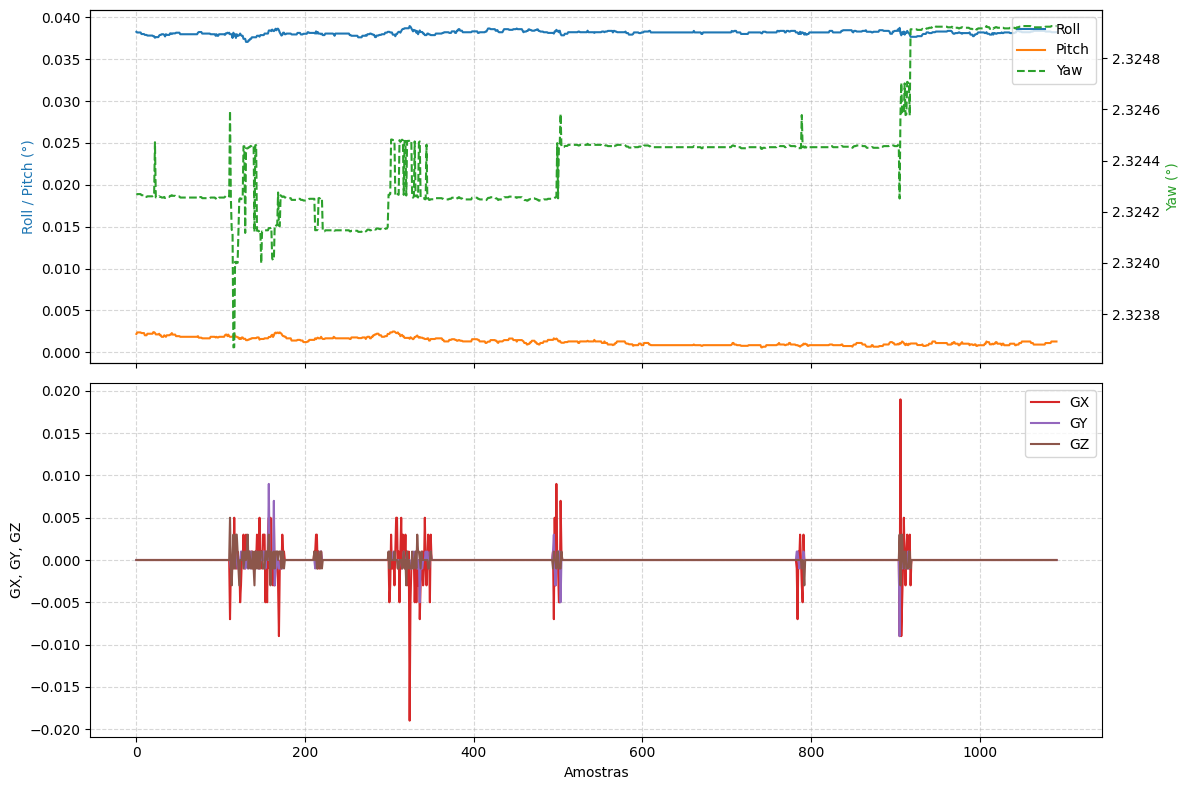
\includegraphics[width=0.85\textwidth]{images/resultados/plotBNO.png}
    \par\vspace{0.2cm}
    \footnotesize Fonte: elaborado pelos autores (2026).
\end{figure}

Com esses dados observados na Figura~\ref{fig:ruido_bno08x}, foi realizada a distribuição estatística do ruído observada em torno do valor médio (ajuste gaussiano).

\begin{figure}[H]
    \centering
    \caption{Distribuição de ruído em roll.}
    \label{fig:dn_roll}
    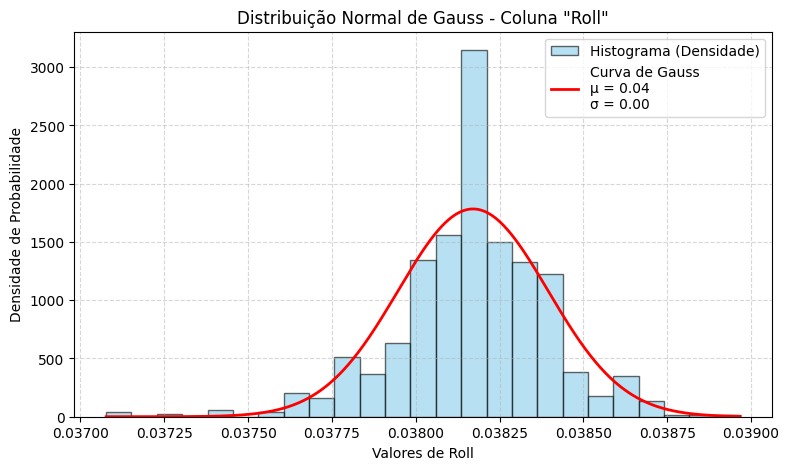
\includegraphics[width=0.85\textwidth]{images/resultados/DNRoll.png}
    \par\vspace{0.2cm}
    \footnotesize Fonte: elaborado pelos autores (2026).
\end{figure}

Observa-se na Figura~\ref{fig:dn_roll} que o sinal apresenta um comportamento compatível com a hipótese de ruído branco gaussiano adotada na formulação do Filtro de Kalman, com desvios contidos em uma faixa estreita em torno da média. Quanto ao determinismo temporal, os carimbos de tempo do \textit{log} mostram que a tarefa de registro no STM32F411 sob FreeRTOS manteve intervalo médio de 100,5~ms (9,95~Hz), com \textit{jitter} (desvio padrão de $\Delta t_i$) de 1,2~ms, intervalos entre 99 e 108~ms e nenhuma lacuna ao longo de aproximadamente 110~s de ensaio. Como o registro foi feito a 10~Hz, uma fração da taxa de 100~Hz dos \textit{reports} SH-2, esses valores descrevem a tarefa de \textit{log}; a taxa efetiva e o \textit{jitter} de cada \textit{report} exigem o registro individual com carimbo de tempo, previsto como etapa seguinte.
Os ensaios foram realizados com os motores desligados. A caracterização da influência da vibração dos motores sobre o ruído da IMU requer um ensaio com os motores em funcionamento, fora do escopo deste ensaio estático.

\subsection{Caracterização do sensor de fluxo óptico e LiDAR MTF-01}\label{subsec:res_mtf01}

De maneira análoga, o módulo MicoAir MTF-01 foi submetido a ensaios estáticos a uma distância vertical fixa de referência em relação ao solo, coletando $N = 729$ amostras consecutivas e operando via interface UART a 115200~bit/s com taxa nominal de saída de aproximadamente 100~Hz, sendo as leituras registradas a 10~Hz pelo \textit{log} USB. O contador de quadros recebidos avançou em média 10,04 quadros por intervalo de registro de 100~ms, o que corresponde a uma taxa efetiva de cerca de 100~Hz, sem erros de CRC, lacunas de sequência, erros de UART ou bytes descartados. A Figura~\ref{fig:bancada_mtf01} mostra o sensor fixado em um suporte provisório durante esse ensaio.

\begin{figure}[H]
    \centering
    \caption{Montagem provisória do sensor MTF-01 para o ensaio de bancada.}
    \label{fig:bancada_mtf01}
    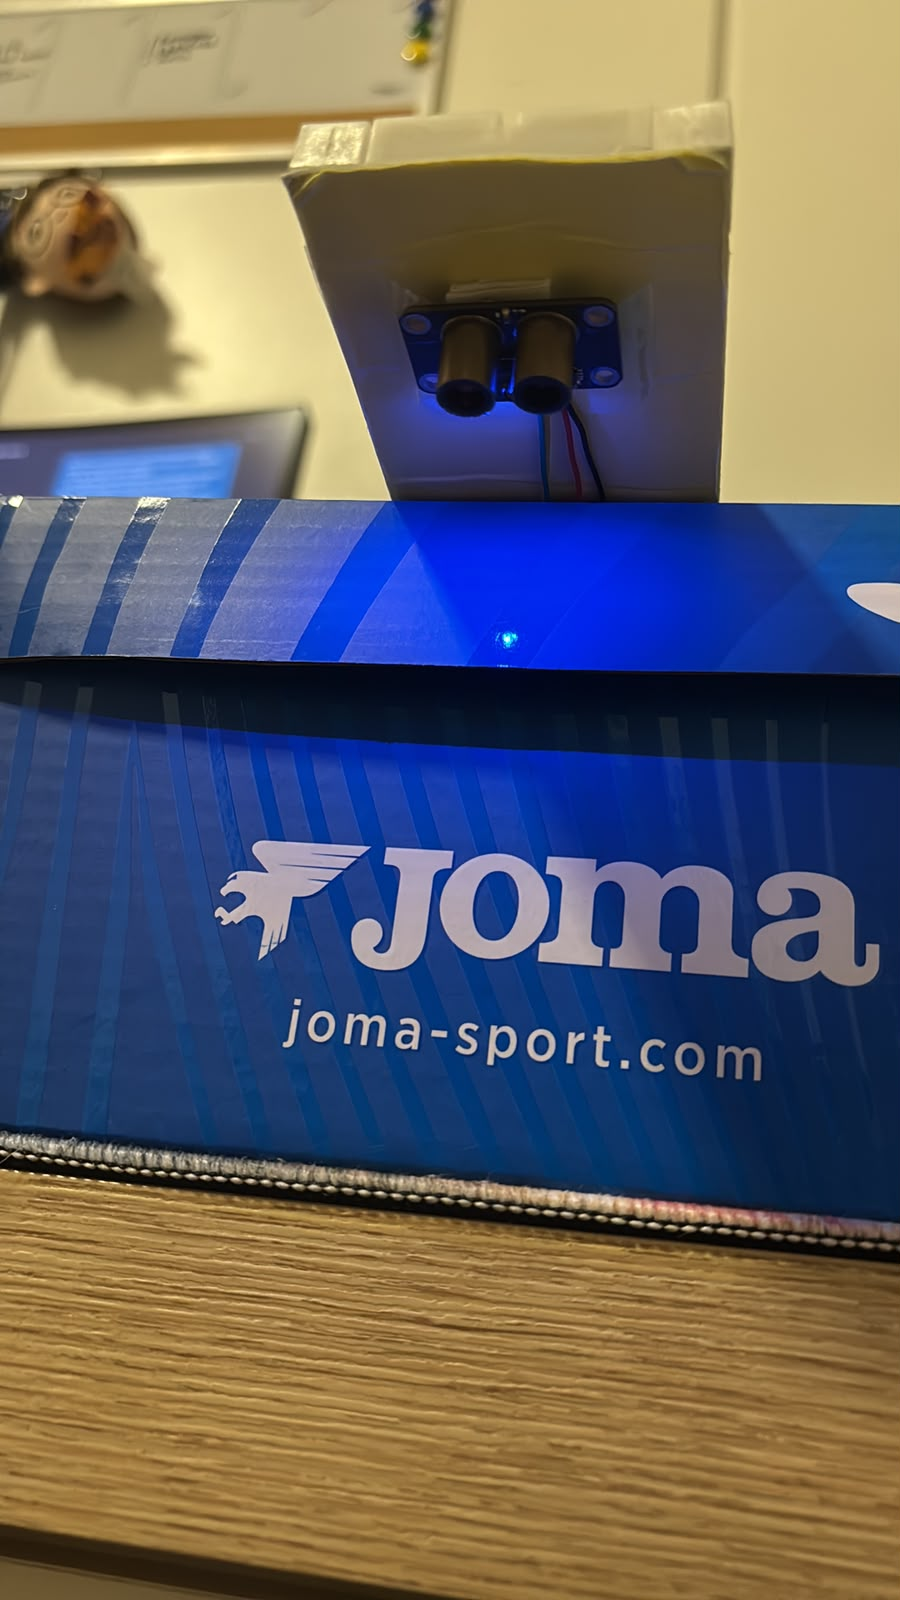
\includegraphics[width=0.4\textwidth]{images/testes/mtf01-bancada.png}
    \par\vspace{0.2cm}
    \footnotesize Fonte: elaborado pelos autores (2026).
\end{figure}

A Figura~\ref{fig:ruido_mtf01} ilustra as séries temporais obtidas para a medição de distância do sensor ToF ($z$) e para as componentes de velocidade linear horizontal ($\dot{x}$ e $\dot{y}$) derivadas do fluxo óptico.

\begin{figure}[H]
    \centering
    \caption{Caracterização experimental de ruído das medições do sensor MTF-01.}
    \label{fig:ruido_mtf01}
    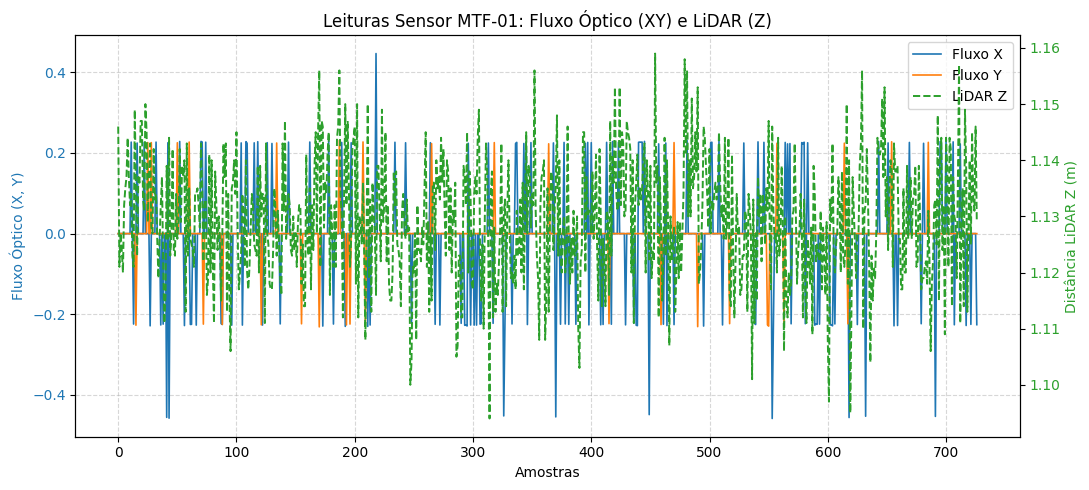
\includegraphics[width=0.85\textwidth]{images/resultados/plotMTF01.png}
    \par\vspace{0.2cm}
    \footnotesize Fonte: elaborado pelos autores (2026).
\end{figure}

Analisando a distribuição de ruído das medições do MTF-01 (Figura~\ref{fig:dn_xyz}), verificou-se que o comportamento estatístico das variáveis $z$, $\dot{x}$ e $\dot{y}$ também se aproxima de uma distribuição gaussiana, com desvios padrão relativamente baixos, indicando boa estabilidade e confiabilidade do sensor em condições estáticas.

\begin{figure}[H]
    \centering
    \caption{Distribuição de ruído em $z$, $\dot{x}$ e $\dot{y}$.}
    \label{fig:dn_xyz}
    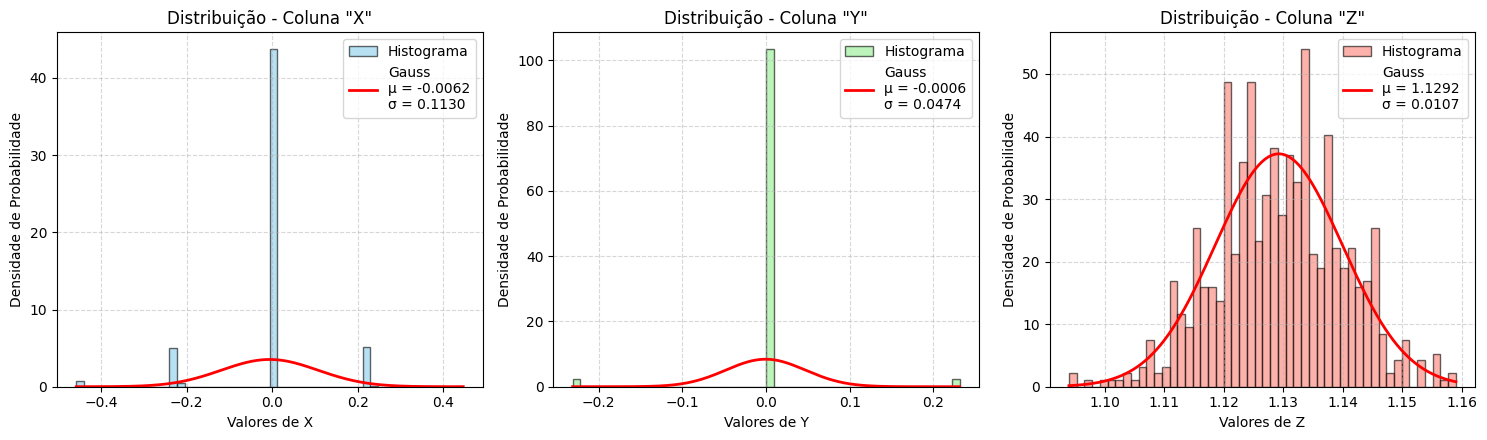
\includegraphics[width=0.85\textwidth]{images/resultados/DNXYZ.png}
    \par\vspace{0.2cm}
    \footnotesize Fonte: elaborado pelos autores (2026).
\end{figure}

O Quadro~\ref{qua:estatistica_sensores} consolida os parâmetros estatísticos extraídos dos ensaios de bancada para ambos os sensores, discriminando a média amostral (\textit{bias} residual), o desvio padrão ($\sigma_v$) e a variância resultante ($\sigma_v^2$) adotada na construção da diagonal da matriz $\mathbf{R}_v$.


\begin{quadro}[H]
\centering
\caption{Parâmetros estatísticos medidos nos sensores e variâncias aplicadas à matriz $\mathbf{R}_v$.}
\label{qua:estatistica_sensores}
\small
\renewcommand{\arraystretch}{1.25}
\setlength{\tabcolsep}{5pt} % Reduz suavemente o espaçamento horizontal entre as colunas
\begin{tabular}{|l|c|c|c|c|c|}
\hline
\textbf{Variável Medida} & \textbf{Sensor} & \textbf{Unidade} & \textbf{\shortstack{Média\\(\textit{Bias})}} & \textbf{\shortstack{Desvio Padrão\\($\sigma_v$)}} & \textbf{\shortstack{Variância\\($\sigma_v^2$)}} \\
\hline
Altitude ($z$) & MTF-01 & m & 1{,}1300 & $1{,}07 \times 10^{-2}$ & $1{,}15 \times 10^{-4}$ \\
Velocidade em $x$ ($\dot{x}$) & MTF-01 & m/s & 0{,}0000 & $1{,}13 \times 10^{-1}$ & $1{,}28 \times 10^{-2}$ \\
Velocidade em $y$ ($\dot{y}$) & MTF-01 & m/s & 0{,}0000 & $4{,}74 \times 10^{-2}$ & $2{,}20 \times 10^{-3}$ \\
Rolamento ($\phi$) & BNO08X & rad & 0{,}0382 & $2{,}24 \times 10^{-4}$ & $5{,}00 \times 10^{-8}$ \\
Arfagem ($\theta$) & BNO08X & rad & 0{,}0013 & $4{,}40 \times 10^{-4}$ & $1{,}94 \times 10^{-7}$ \\
Guinada ($\psi$) & BNO08X & rad & 2{,}3245 & $2{,}46 \times 10^{-4}$ & $6{,}04 \times 10^{-8}$ \\
Taxa de rolamento ($p$) & BNO08X & rad/s & 0{,}0000 & $1{,}44 \times 10^{-3}$ & $2{,}06 \times 10^{-6}$ \\
Taxa de arfagem ($q$) & BNO08X & rad/s & 0{,}0000 & $5{,}70 \times 10^{-4}$ & $3{,}24 \times 10^{-7}$ \\
Taxa de guinada ($r$) & BNO08X & rad/s & 0{,}0000 & $4{,}88 \times 10^{-4}$ & $2{,}38 \times 10^{-7}$ \\
\hline
\end{tabular}
\par\vspace{0.2cm}
\footnotesize Fonte: elaborado pelos autores (2026).
\end{quadro}

% =============================================================
\section{SIMULAÇÕES EM AMBIENTE MATLAB/SIMULINK}\label{sec:res_simulacoes}

Para realizar a validação do projeto de controle LQG antes dos ensaios de voo livre, foram conduzidas simulações numéricas no ambiente MATLAB/Simulink (versão R2024a). Primeiramente, implementou-se o modelo linearizado do quadricóptero em torno da condição de \textit{hover}, fundamentado nas matrizes de espaço de estados derivadas na Seção~\ref{subsubsec:linearizacao_sistema}, com a finalidade de verificar as propriedades estruturais de controlabilidade, observabilidade e estabilidade em malha fechada, além de sintonizar as matrizes de ponderação $\mathbf{Q}$ e $\mathbf{R}_{\mathrm{lqr}}$. Na sequência, o mesmo compensador LQG e os mesmos ganhos ($\mathbf{K}$ e $\mathbf{L}$) foram aplicados ao modelo dinâmico completo não linear do quadricóptero, incorporando os acoplamentos inerciais, as não linearidades trigonométricas e o ruído estocástico parametrizado pelo Quadro~\ref{qua:estatistica_sensores}.

\subsection{Verificação estrutural e sintonia das matrizes do controlador}\label{subsec:res_sintonia}

A verificação algébrica preliminar do par $(\mathbf{A}, \mathbf{B})$ confirmou o posto completo da matriz de controlabilidade ($\operatorname{rank}(\mathcal{C}) = 12$). Por outro lado, o par $(\mathbf{A}, \mathbf{C})$ apresentou deficiência de posto na matriz de observabilidade ($\operatorname{rank}(\mathcal{O}) = 10$), indicando que o sistema é completamente controlável nos 12 estados, porém não é observável nas posições translacionais $x$ e $y$ devido à ausência de medições de posição absoluta no plano horizontal. Dessa forma, comprova-se a necessidade da aplicação de um estimador de estados ótimo, como o Filtro de Kalman, para realizar a fusão sensorial, atenuar ruídos de medição e reconstruir dinamicamente o subsistema observável.

Após o processo iterativo de ajuste baseado no compromisso entre velocidade de resposta e limitação de esforço nos atuadores, definiram-se os seguintes valores para as diagonais das matrizes de ponderação de estados ($\mathbf{Q}$) e de controle ($\mathbf{R}_{\mathrm{lqr}}$):

\begin{equation}\label{eq:valores_Q_R_sim}
\begin{aligned}
\mathbf{Q} &= \operatorname{diag}\left(5,\, 5,\, 500,\, 500,\, 500,\, 50,\, 5,\, 5,\, 5,\, 10,\, 10,\, 5\right), \\
\mathbf{R}_{\mathrm{lqr}} &= \operatorname{diag}\left(0{,}1,\, 0{,}1,\, 0{,}1,\, 0{,}1\right).
\end{aligned}
\end{equation}

Todos os autovalores das matrizes de malha fechada do regulador ($\mathbf{A} - \mathbf{B}\mathbf{K}$) e do observador ($\mathbf{A} - \mathbf{L}\mathbf{C}$) posicionaram-se estritamente no semiplano esquerdo do plano complexo (ou no interior do círculo unitário, na formulação discreta com período de amostragem $T_s = 100$~ms), confirmando a estabilidade assintótica local do sistema.

\subsection{Desempenho do Filtro de Kalman na estimação de estados}\label{subsec:res_kalman}

A eficácia do Filtro de Kalman na rejeição do ruído de medição foi avaliada comparando-se os estados reais da planta, os sinais corrompidos pelo ruído sensorial ($\mathbf{y}$) e os estados reconstruídos pelo estimador ($\hat{\mathbf{x}}$). A Figura~\ref{fig:simulacao_kalman} apresenta a sobreposição entre a leitura ruidosa e a estimativa filtrada para as variáveis do sistema.

\begin{figure}[H]
    \centering
    \caption{Comparação entre estados reais, medições ruidosas e estimativas do Filtro de Kalman.}
    \label{fig:simulacao_kalman}
    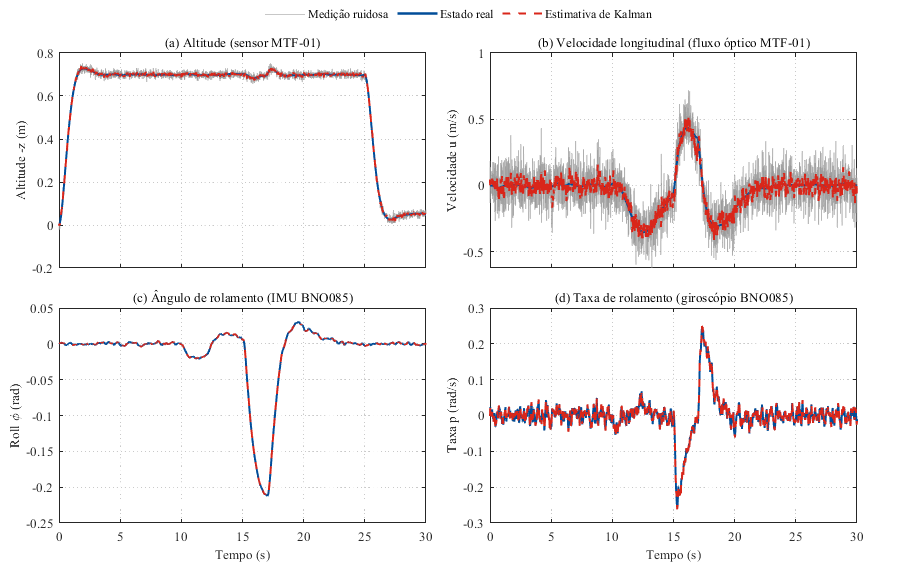
\includegraphics[width=0.85\textwidth]{images/resultados/kalman.png}
    \par\vspace{0.2cm}
    \footnotesize Fonte: elaborado pelos autores (2026).
\end{figure}

Verifica-se na Figura~\ref{fig:simulacao_kalman} que o estimador atenua significativamente as flutuações de alta frequência oriundas dos sensores sem introduzir atraso de fase excessivo na malha, fornecendo uma estimativa suave ($\hat{\mathbf{x}}$) para o cálculo da lei de controle LQR e evitando que o ruído de medição seja amplificado pelos ganhos da matriz $\mathbf{K}$ nos comandos enviados aos motores.

\subsection{Comparação entre o modelo linear e o modelo não linear}\label{subsec:res_linear_vs_naolinear}

Para avaliar o domínio de validade da linearização por série de Taylor e a robustez do controlador LQG frente às dinâmicas não lineares do quadricóptero, ambos os modelos foram submetidos às mesmas condições iniciais e perfis de referência. O ensaio consiste em inicializar a aeronave na origem do referencial inercial, $[x,\, y,\, z]^{\top} = [0,\, 0,\, 0]^{\top}\text{ m}$, comandando-se inicialmente uma manobra de subida para a altitude de $0{,}7\text{ m}$. Em seguida, aplica-se uma rotação de $45^\circ$ ($\pi/4\text{ rad}$) em torno do eixo de guinada ($\psi$) em $t = 5\text{ s}$ e, posteriormente, um deslocamento translacional no plano horizontal em $t = 10\text{ s}$ (suavizado por um limitador de taxa) até as coordenadas de magnitude $[1{,}0,\, 1{,}0]\text{ m}$. Após a estabilização, o sistema é submetido, entre $t = 15\text{ s}$ e $t = 17\text{ s}$, a um distúrbio externo de atitude equivalente a $10^\circ$ em rolamento ($\phi$), $-5^\circ$ em arfagem ($\theta$) e $10^\circ$ em guinada ($\psi$), devendo rejeitar a perturbação e retomar a atitude de equilíbrio. Por fim, em $t = 25\text{ s}$, executa-se a manobra de redução de altitude (pouso).

A Figura~\ref{fig:comp_atitude} apresenta a resposta transitória comparativa dos ângulos de atitude ($\phi$, $\theta$ e $\psi$) entre o modelo linear e o modelo não linear, a Figura~\ref{fig:comp_posicaoXY} exibe o rastreamento de posição $x$ e $y$, e por fim a Figura~\ref{fig:comp_posicaoZ} mostra o rastreamento de posição $z$.

\begin{figure}[H]
    \centering
    \caption{Comparação da resposta de atitude ($\phi, \theta, \psi$): modelo linear vs. modelo não linear.}
    \label{fig:comp_atitude}
    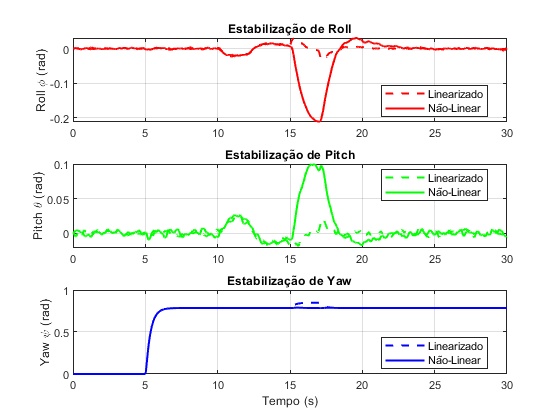
\includegraphics[width=0.85\textwidth]{images/resultados/comparacao_atitude.png}
    \par\vspace{0.2cm}
    \footnotesize Fonte: elaborado pelos autores (2026).
\end{figure}

\begin{figure}[H]
    \centering
    \caption{Comparação da resposta de posição ($x, y, z$): modelo linear vs. modelo não linear.}
    \label{fig:comp_posicaoXY}
    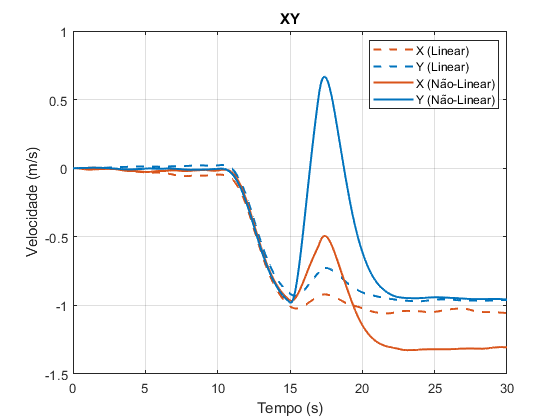
\includegraphics[width=0.85\textwidth]{images/resultados/comparacao_posicaoXY.png}
    \par\vspace{0.2cm}
    \footnotesize Fonte: elaborado pelos autores (2026).
\end{figure}

\begin{figure}[H]
    \centering
    \caption{Comparação da resposta de posição ($x, y, z$): modelo linear vs. modelo não linear.}
    \label{fig:comp_posicaoZ}
    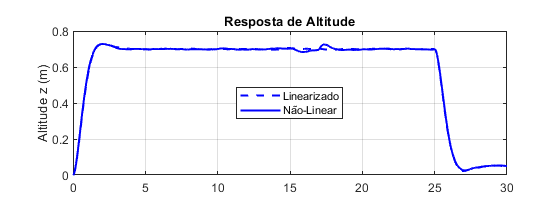
\includegraphics[width=0.85\textwidth]{images/resultados/comparacao_posicaoZ.png}
    \par\vspace{0.2cm}
    \footnotesize Fonte: elaborado pelos autores (2026).
\end{figure}

Adicionalmente, a Figura~\ref{fig:esforco_motores} ilustra o comportamento das velocidades angulares comandadas aos quatro rotores ($\omega_1, \omega_2, \omega_3, \omega_4$) durante a manobra, demonstrando que as ações de controle convergem para a rotação nominal de equilíbrio ($\omega_0 \approx 146{,}23$~rad/s) e permanecem dentro dos limites físicos de saturação dos propulsores.

\begin{figure}[H]
    \centering
    \caption{Velocidades angulares comandadas aos quatro motores ($\omega_1$ a $\omega_4$) na simulação.}
    \label{fig:esforco_motores}
    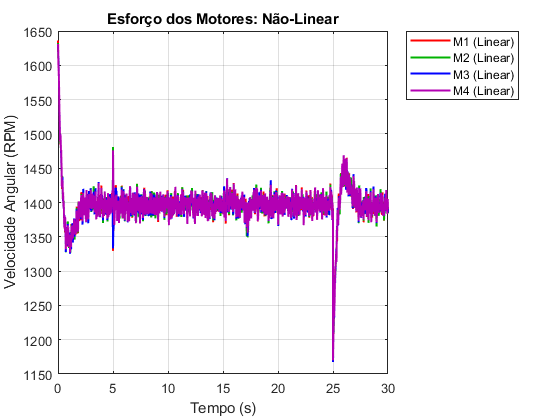
\includegraphics[width=0.85\textwidth]{images/resultados/esforco_motores.png}
    \par\vspace{0.2cm}
    \footnotesize Fonte: elaborado pelos autores (2026).
\end{figure}

Para quantificar objetivamente a aderência entre a aproximação linear e a planta não linear, conforme definido na Seção~\ref{subsec:metricas_lqr}, o Quadro~\ref{qua:metricas_simulacao} resume os indicadores de desempenho obtidos para cada grau de liberdade: Raiz do Erro Quadrático Médio (RMSE), Erro Absoluto Médio (MAE), sobressinal percentual ($M_p$), tempo de acomodação ($t_s$ para banda de 2\%) e erro em regime permanente ($e_{\mathrm{ss}}$).

\begin{quadro}[H]
\centering
\caption{Comparativo das métricas de desempenho de controle entre o modelo linear e o não linear.}
\label{qua:metricas_simulacao}
\small
\renewcommand{\arraystretch}{1.25}
\setlength{\tabcolsep}{5pt} % Reduz levemente o espaçamento horizontal entre as colunas
\begin{tabular}{|l|c|c|c|c|c|c|}
\hline
\textbf{Variável / Modelo} & \textbf{Unid.} & \textbf{RMSE} & \textbf{MAE} & \textbf{\shortstack{Sobressinal\\($M_p$)}} & \textbf{\shortstack{Acomodação\\($t_s$)}} & \textbf{\shortstack{Erro Estac.\\($e_{\mathrm{ss}}$)}} \\
\hline
\multicolumn{7}{|l|}{\textbf{Modelo Linearizado}} \\
\hline
Posição $x$ & m & 0,289 & 0,205 & 0,0\% & 14,90~s & 0,073 \\
Posição $y$ & m & 0,271 & 0,177 & 2,5\% & 14,90~s & 0,023 \\
Altitude $z$ & m & 0,098 & 0,022 & 4,2\% & 2,73~s & 0,002 \\
Rolamento ($\phi$) & graus & 0,633 & 0,447 & 1,7$^\circ$\textsuperscript{*} & 2,95~s & 0,009 \\
Arfagem ($\theta$) & graus & 0,543 & 0,410 & 1,6$^\circ$\textsuperscript{*} & 2,93~s & 0,282 \\
Guinada ($\psi$) & graus & 6,385 & 1,630 & 0,0\% & 1,27~s & 0,001 \\
\hline
\multicolumn{7}{|l|}{\textbf{Modelo Não Linear Completo}} \\
\hline
Posição $x$ & m & 0,363 & 0,313 & 29,4\% & 14,90~s & 0,285 \\
Posição $y$ & m & 0,725 & 0,544 & 0,0\% & 14,90~s & 0,132 \\
Altitude $z$ & m & 0,097 & 0,023 & 4,2\% & 17,69~s & 0,001 \\
Rolamento ($\phi$) & graus & 3,931 & 2,082 & 12,2$^\circ$\textsuperscript{*} & 6,41~s & 0,040 \\
Arfagem ($\theta$) & graus & 1,955 & 1,162 & 6,0$^\circ$\textsuperscript{*} & 5,63~s & 0,005 \\
Guinada ($\psi$) & graus & 6,387 & 1,632 & 0,0\% & 1,27~s & 0,003 \\
\hline
\end{tabular}
\par\vspace{0.15cm}
\footnotesize \textsuperscript{*}Para $\phi$ e $\theta$ (regulação em $0^\circ$), $M_p$ representa a deflexão angular máxima absoluta atingida nas manobras e rejeição de distúrbios.\\
Fonte: elaborado pelos autores (2026).
\end{quadro}

A análise comparativa das curvas e das métricas do Quadro~\ref{qua:metricas_simulacao} demonstra que, dentro do envelope operacional de pequenos ângulos ($|\phi|, |\theta| \le 15^\circ$), as respostas dos modelos linear e não linear apresentam elevada concordância. As pequenas divergências observadas durante os instantes iniciais do regime transitório no modelo não linear devem-se ao termo de acoplamento trigonométrico do empuxo ($\cos\phi\cos\theta$) na dinâmica vertical e aos termos giroscópicos cruzados nas equações rotacionais, os quais são prontamente compensados pela malha fechada LQG sem comprometer a estabilidade do sistema.

Graficamente se observa um grande desvio nas posições $x$ e $y$ do modelo não linear, no momento que ocorre o distúrbio. Após a tentativa de estabilização, acaba ocorrendo um erro de regime permanente, que é explicado pela falta de observabilidade das posições horizontais, uma vez que o sistema não possui sensores de posição absoluta. Por outro lado, a altitude $z$ e os ângulos de atitude ($\phi$, $\theta$, $\psi$) apresentam excelente rastreamento e rejeição de distúrbios, com erros em regime permanente desprezíveis.

\section{Validação em Voo Real}\label{sec:resultados_voo}

Após a calibração do Filtro de Kalman e a validação teórica das matrizes de ganho do controlador ótimo em ambiente de simulação, procedeu-se aos ensaios práticos de voo. O objetivo desta etapa consistiu em avaliar a capacidade do controlador LQR/LQG embarcado em manter o quadricóptero estabilizado na origem do plano horizontal ($X=0, Y=0$) e na altitude de referência de $15\,\mathrm{cm}$. Os dados telemétricos foram transmitidos via interface serial e gravados com uma taxa de amostragem de $50\,\mathrm{Hz}$.

A Figura \ref{fig:telemetria_atitude} apresenta a resposta temporal do sistema em malha fechada para as variáveis de atitude (rolamento, arfagem e guinada), a altitude em relação ao solo e o respectivo esforço de controle aplicado aos atuadores. A decolagem autônoma ocorreu aproximadamente no instante $t = 7\,\mathrm{s}$.

\begin{figure}[H]
\centering
\caption{Telemetria completa do voo: atitude, altitude e esforço de controle.}
\label{fig:telemetria_atitude}
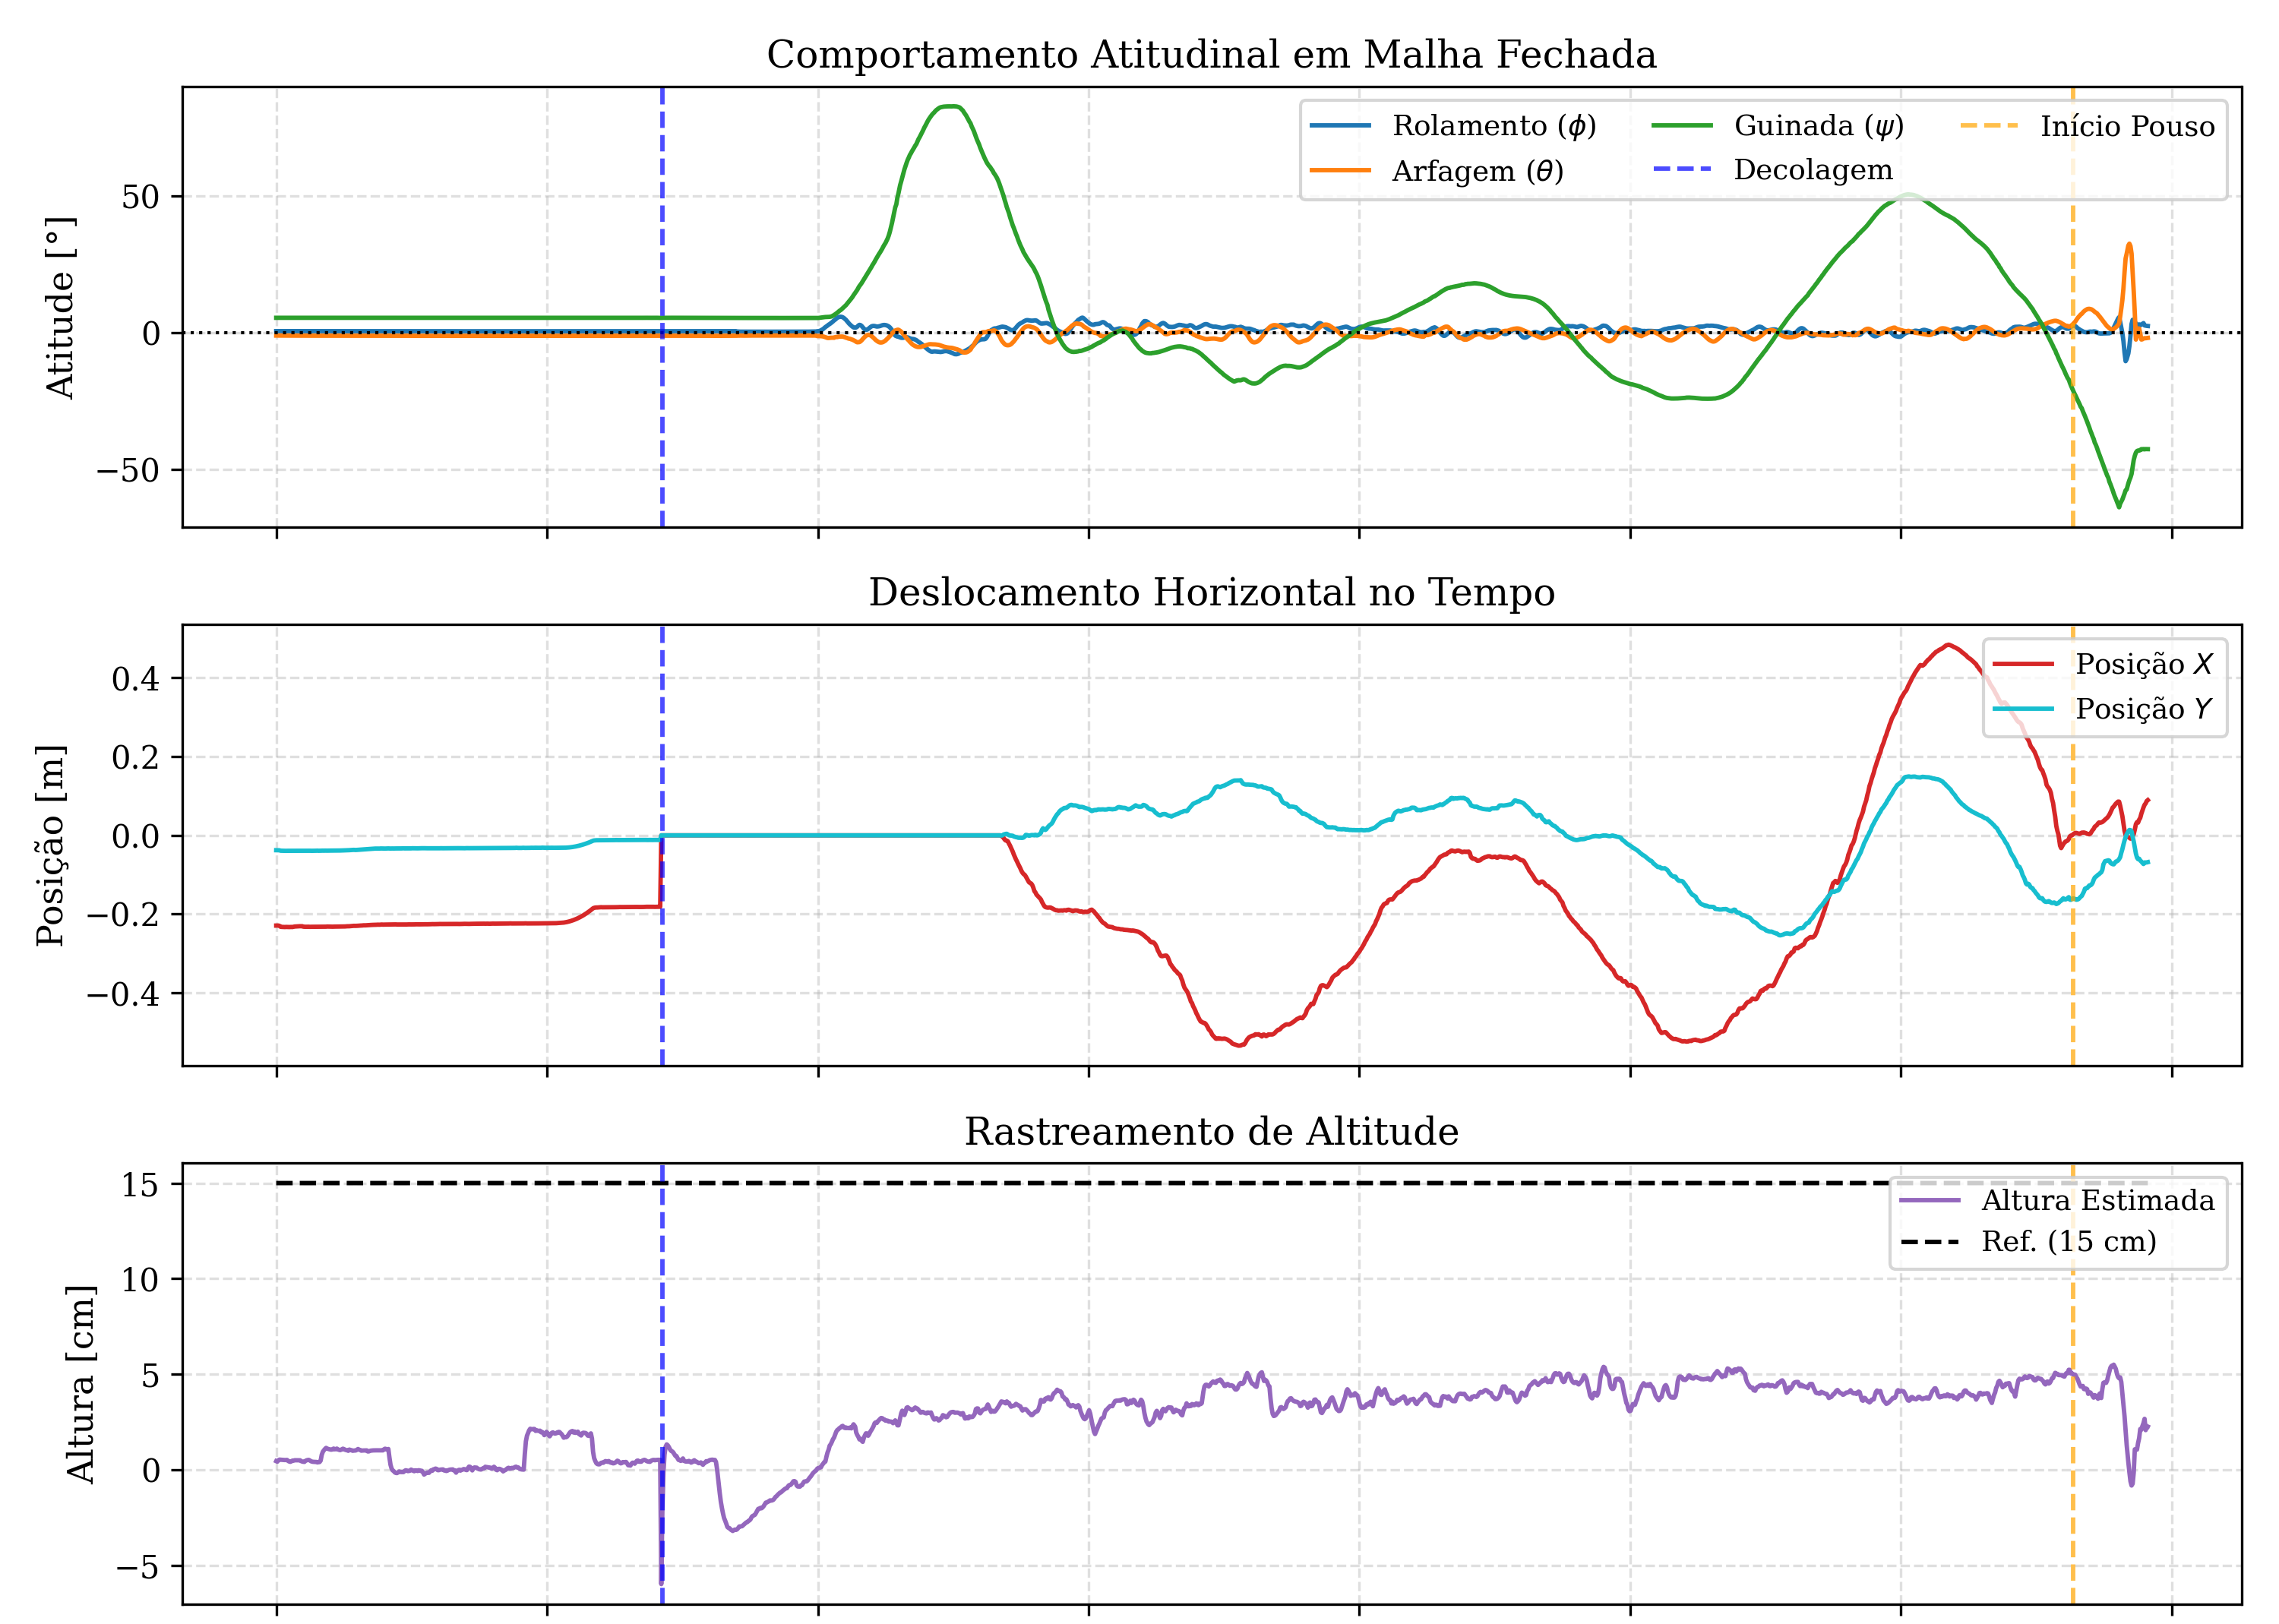
\includegraphics[width=0.9\textwidth]{images/resultados/telemetria_voo_completa.png}
\vspace{0.2cm}
\par\footnotesize Fonte: elaborado pelos autores (2026).
\end{figure}

A análise das curvas de atitude revela que o controlador foi capaz de manter os ângulos de rolamento ($\phi$) e arfagem ($\theta$) estabilizados em uma faixa estreita de oscilação em torno de suas referências, mesmo sob os ruídos mecânicos de alta frequência gerados pelos propulsores. A guinada ($\psi$), por outro lado, não foi regulada, variando entre aproximadamente $+80^\circ$ e $-60^\circ$ ao longo do voo. A altura estimada estabilizou-se entre 4 e 5~cm, abaixo da referência de 15~cm. Em ensaios complementares, com o deslocamento horizontal restringido por um apoio físico, a altura de referência foi alcançada, o que indica que a manutenção da posição horizontal na origem é a condição que falta para a subida até a altura de referência em voo livre.

Contudo, apesar da estabilidade de rolamento e arfagem, a malha de controle de posição externa não atingiu o desempenho projetado. A Figura \ref{fig:telemetria_xy} ilustra a trajetória estimada do quadricóptero no plano cartesiano, evidenciando uma oscilação não compensada em torno da origem, com excursões de até cerca de 0,5~m no eixo $X$. 

\begin{figure}[H]
\centering
\caption{Trajetória estimada do veículo no plano horizontal ($X \times Y$).}
\label{fig:telemetria_xy}
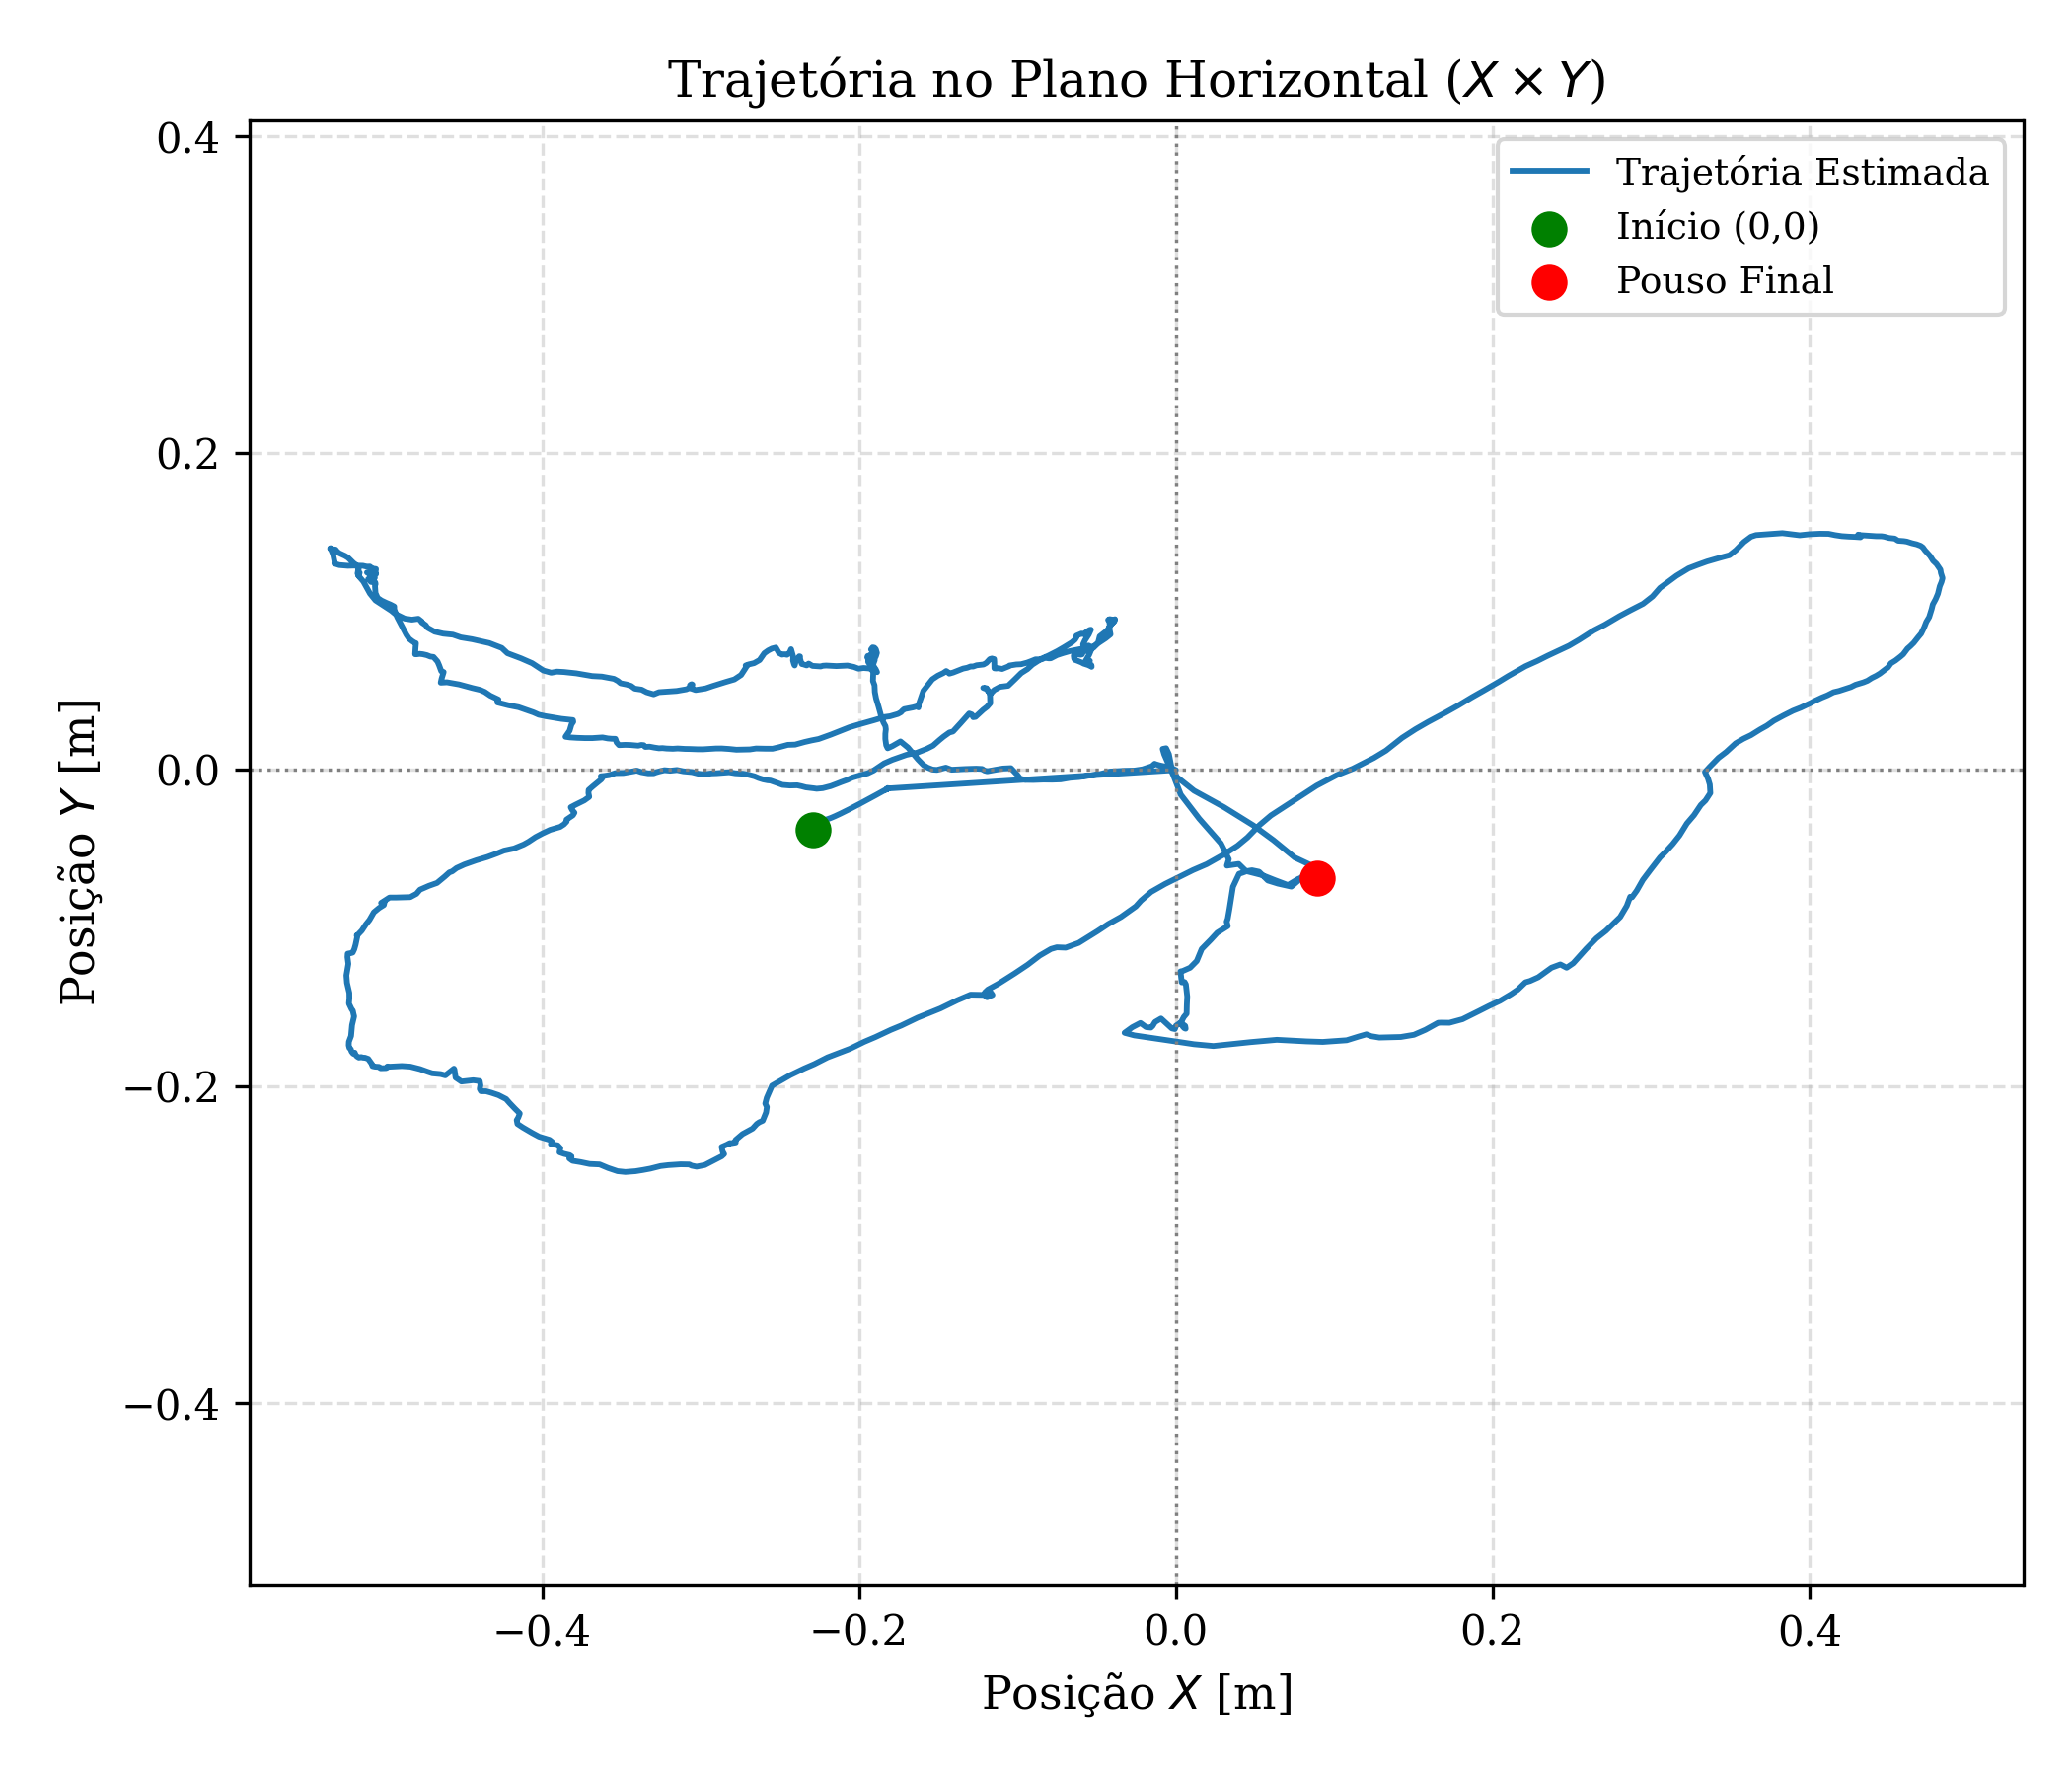
\includegraphics[width=0.7\textwidth]{images/resultados/trajetoria_plano_xy.png}
\vspace{0.2cm}
\par\footnotesize Fonte: elaborado pelos autores (2026).
\end{figure}

Observa-se que, durante a subida em direção à altura de referência, o veículo não manteve a posição horizontal na origem. Ao se deslocar, ficou sujeito a forças externas presentes no ambiente de ensaio, como o cabo USB conectado, a proximidade de paredes, o contato com as mãos do operador ou correntes de ar em espaço aberto, e foram essas forças que o levaram a ultrapassar a inclinação máxima de segurança estabelecida no firmware. Nesse limiar, a supervisão acionou a rotina de pouso seguida do corte dos motores (\textit{failsafe}). Nos ensaios em que nenhuma força externa atuou sobre o veículo, a inclinação de \textit{failsafe} não foi atingida.

A divergência na posição plana, coexistindo com rolamento e arfagem estabilizados, sugere a presença de perturbações externas constantes não modeladas (como um deslocamento do centro de massa em relação à controladora de voo ou correntes de ar) combinadas ao acúmulo de erros de integração (\textit{drift}) típicos do sensor de fluxo óptico MTF-01 ao operar perto do solo. Em trabalhos futuros, a introdução de uma malha adaptativa para estimar o desbalanceamento estático ou o refinamento empírico da matriz de covariância de ruído do processo ($Q$) poderiam mitigar esse comportamento.

\subsection{Registro do voo sem cabo e acompanhamento pelo terminal}
\label{subsec:voo_sem_cabo}

A imagem (a) da Figura~\ref{fig:voo_terminal} registra o protótipo em voo físico, sem cabo conectado ao computador. Esse registro difere dos ensaios de comunicação com o veículo simulado: neste caso, os motores estavam em funcionamento e o drone se deslocava no ambiente real.



O ensaio é iniciado pelo operador no terminal do Raspberry Pi, por meio do programa de teste de voo pairado. O comando \texttt{hover-test}, com a opção \texttt{--motors}, solicita a execução física do teste; as opções \texttt{--height} e \texttt{--time} definem a altura de referência e a duração solicitada. Também podem ser fornecidos parâmetros de controle e uma identificação para o registro. O Raspberry Pi coordena o ensaio e coleta a telemetria, enquanto o STM32 executa o controle do veículo. Ao final, o programa salva o registro no Raspberry Pi e apresenta um resumo no terminal. O encerramento pode ocorrer antes do previsto se uma condição de supervisão interromper o teste.

A imagem (b) da Figura~\ref{fig:voo_terminal} apresenta esse relatório ao final de um teste físico de decolagem. No registro mostrado, a referência era de 15~cm, mas a altura máxima informada foi de 6,3~cm. O programa indicou que o alvo não foi atingido em 26~s e iniciou o pouso, seguido do desarme. Foram registradas 2082 amostras de telemetria a 50~Hz, com 3,2\% de perdas informadas no relatório. Esses dados documentam o acompanhamento do ensaio e a limitação de altitude observada nesse registro; não demonstram que a referência de decolagem tenha sido alcançada.

\begin{figure}[htbp]
    \centering
    \caption{Registro conjunto do ensaio físico: (a) protótipo em voo sem cabo; (b) relatório apresentado no terminal ao término do teste.}
    \label{fig:voo_terminal}
    \begin{minipage}[t]{0.48\textwidth}
        \centering
        \vspace{0pt}
        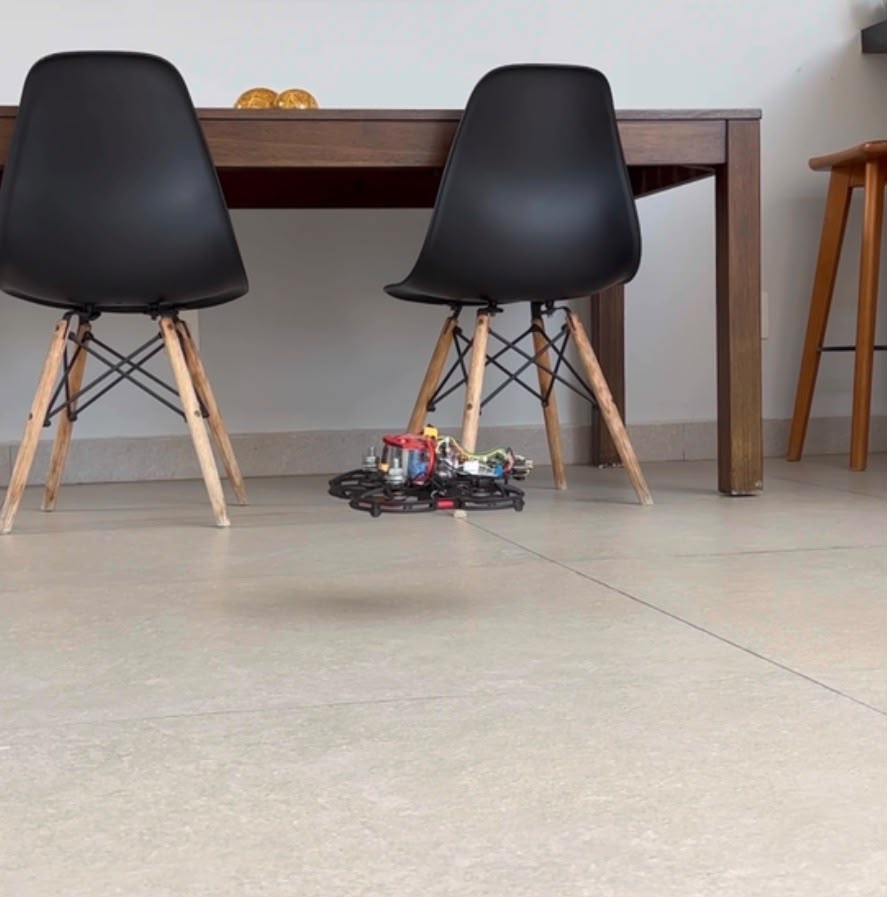
\includegraphics[width=\linewidth,height=8cm,keepaspectratio]{images/resultados/drone_sem_fio.jpeg}
        \par\smallskip{\footnotesize (a) Protótipo em voo.}
    \end{minipage}
    \hfill
    \begin{minipage}[t]{0.48\textwidth}
        \centering
        \vspace{0pt}
        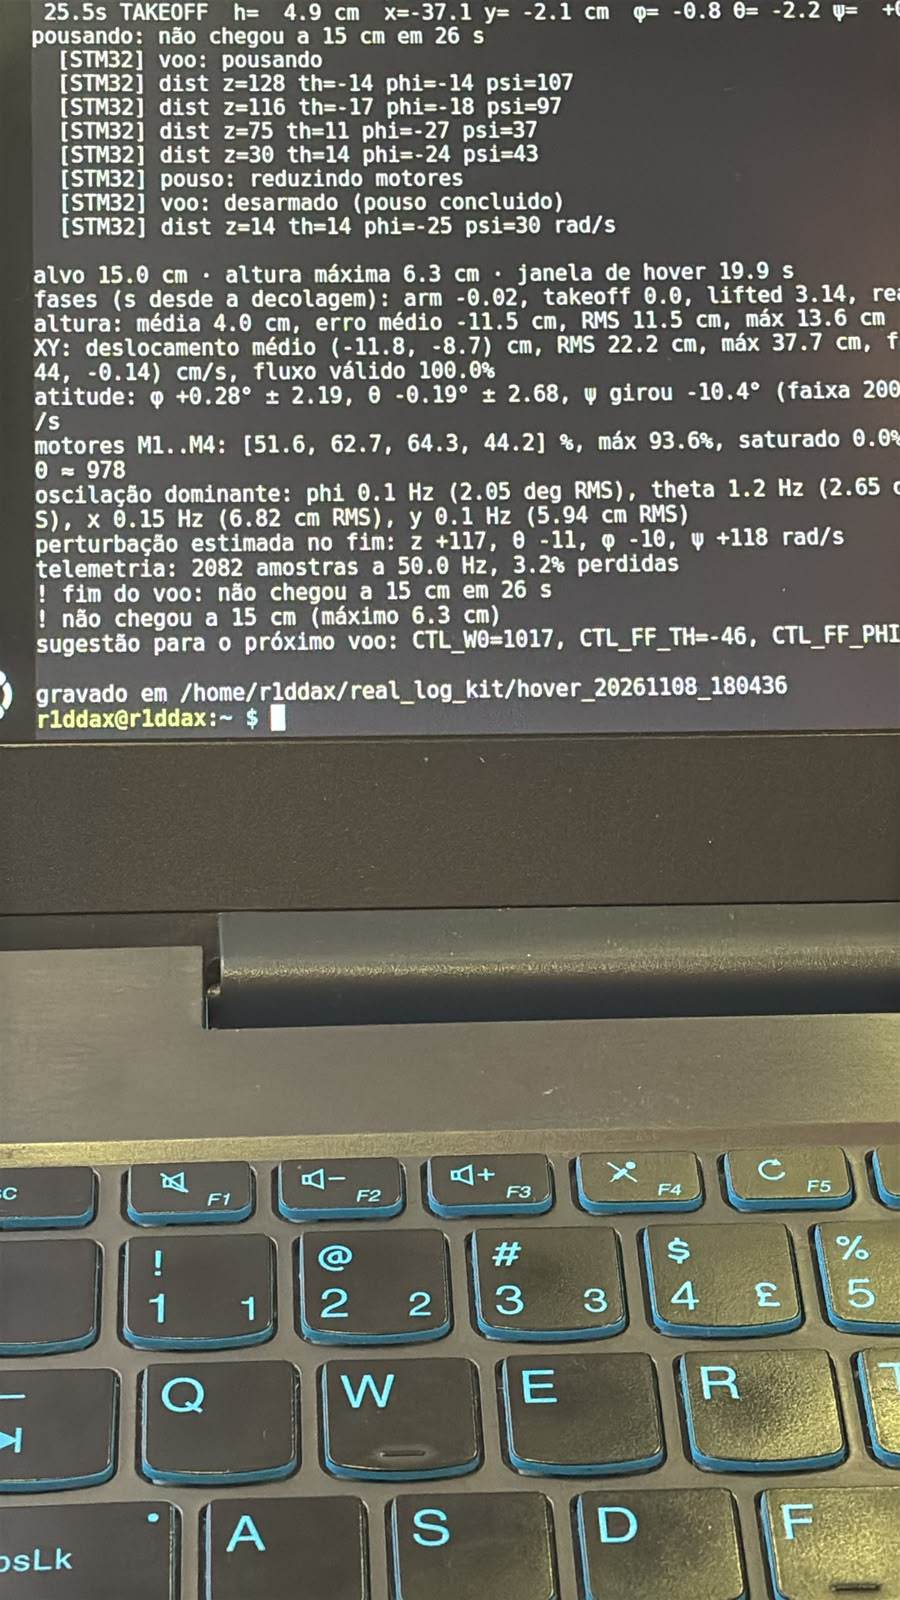
\includegraphics[width=\linewidth,height=8cm,keepaspectratio]{images/resultados/terminal.jpeg}
        \par\smallskip{\footnotesize (b) Relatório do ensaio.}
    \end{minipage}
    \par\vspace{0.2cm}
    \footnotesize Fonte: elaborado pelos autores (2026).
\end{figure}

% Comunicação Raspberry Pi <-> STM32 (testes, ensaios no STM32, problemas corrigidos)
% ============================================================================
% RESULTADOS — comunicação entre o Raspberry Pi e o STM32 (DroneLink)
% Chamado em partes/textuais/resultados.tex.
% Registro do ensaio: DroneSTM32/docs/resultados_comunicacao/
%   dronelink_20261107_225922.json (tools/pi/ensaios/ensaio_dronelink.py).
% ============================================================================

\section{COMUNICAÇÃO ENTRE O COMPUTADOR DE MISSÃO E O CONTROLADOR DE VOO}\label{sec:res_comunicacao}

Esta seção apresenta os resultados dos três níveis de ensaio descritos na Seção~\ref{subsubsec:com_ensaios}. O ensaio integrado foi realizado com o Raspberry Pi Zero W ligado ao STM32 pela UART, com o VANT simulado no STM32 (\texttt{FLT\_SIM = 1}) e os motores parados. Também são relatados os problemas encontrados e corrigidos durante a integração.

% ----------------------------------------------------------------
\subsection{Testes automatizados}\label{subsec:res_com_testes}
% ----------------------------------------------------------------

A Tabela~\ref{tab:com_testes} apresenta as verificações automatizadas do \texttt{dronectl}, realizadas com um STM32 simulado em Python. Os testes compararam as respostas e os estados obtidos com os resultados esperados. Os casos apresentados foram executados com sucesso no computador pessoal e no Raspberry Pi.

\begin{table}[H]
    \centering
    \caption{Testes do programa \texttt{dronectl} simulado.}
    \label{tab:com_testes}
    \small
    \renewcommand{\arraystretch}{1.25}
    \begin{tabular}{p{4.5cm}p{9.3cm}}
        \hline
        \textbf{Teste} & \textbf{O que verifica} \\
        \hline
        Sequência de voo &
        Armamento, decolagem, recebimento de telemetria e dados de depuração, pouso e retorno ao estado desarmado. \\
        Parâmetros &
        Leitura e alteração de parâmetros e recebimento do valor adotado pelo simulador. \\
        Envio de ganhos &
        Envio dos ganhos do LQG, retransmissão de uma linha perdida e confirmação do CRC-32. \\
        Interpretação dos comandos &
        Aceitação de comandos válidos e recusa de comandos, números e pontos inválidos. \\
        Cálculo do trecho &
        Cálculo da distância e do menor giro até um ponto. \\
        Movimento antes da decolagem &
        A ferramenta não envia um comando de movimento enquanto o veículo simulado está no chão. \\
        Trecho fora de \texttt{HOLD} &
        Um trecho enviado diretamente ao simulador fora de \texttt{HOLD} é recusado. \\
        Missão com comandos manuais &
        Execução de comandos de decolagem, giro, deslocamento, visita a pontos e pouso. \\
        Rotas em 2D e 3D &
        Execução de \texttt{route} com retorno ao ponto de partida. \\
        Missão por arquivo &
        Leitura e execução da missão de um quadrado de 40~cm. \\
        Resposta antiga &
        Uma resposta de outra missão não encerra o trecho atual. \\
        Erro durante a missão &
        Um comando inválido interrompe a missão e a ferramenta solicita o pouso. \\
        \hline
    \end{tabular}
    \par\vspace{0.2cm}
    \footnotesize Fonte: elaborado pelos autores (2026).
\end{table}

Foram executadas nove suítes de teste de módulos do \textit{firmware} no computador, compiladas com o GCC e os recursos AddressSanitizer e UndefinedBehaviorSanitizer, para detectar determinados erros de memória e comportamentos indefinidos. Na versão avaliada, o \textit{firmware} ocupou 106~kB dos 512~kB de \textit{Flash} (21\%) e 80~kB dos 128~kB de RAM (63\%) do STM32F411.

% ----------------------------------------------------------------
\subsection{Enlace UART entre o Raspberry Pi e o STM32}\label{subsec:res_com_enlace}
% ----------------------------------------------------------------

A Tabela~\ref{tab:com_enlace} apresenta o tráfego recebido pelo Raspberry Pi durante 60~s, com o VANT simulado e os motores parados. As taxas medidas ficaram próximas das configuradas. No período, não foram registradas perdas de mensagens nem erros de \textit{checksum}. Quatro mensagens foram recebidas fora de ordem, sem serem contabilizadas como perdas.

\begin{table}[H]
    \centering
    \caption{Tráfego do STM32 recebido pelo Raspberry Pi em 60~s, com o VANT parado.}
    \label{tab:com_enlace}
    \small
    \renewcommand{\arraystretch}{1.2}
    \begin{tabular}{lcc}
        \hline
        \textbf{Mensagem} & \textbf{Taxa nominal} & \textbf{Taxa medida} \\
        \hline
        \texttt{HEARTBEAT} & 2~Hz & 1,98~Hz \\
        \texttt{SYS\_STATUS} & 2~Hz & 2,00~Hz \\
        \texttt{DRONE\_PROTOCOL\_INFO} & 1~Hz & 1,00~Hz \\
        \texttt{ATTITUDE} & 5~Hz & 4,97~Hz \\
        \texttt{LOCAL\_POSITION\_NED} & 5~Hz & 4,97~Hz \\
        \hline
        \multicolumn{3}{l}{895 mensagens; 552~B/s; 0 perdidas; 0 erros de \textit{checksum}; 4 fora de ordem} \\
        \hline
    \end{tabular}
    \par\vspace{0.2cm}
    \footnotesize Fonte: elaborado pelos autores (2026).
\end{table}

O tráfego médio de 552~bytes/s correspondeu a aproximadamente 4,8\% da capacidade do enlace no sentido do STM32 para o Raspberry Pi. Em 100 leituras de parâmetro, a latência de ida e volta apresentou mediana de 10,2~ms e máximo de 21,2~ms. Esses resultados foram compatíveis com a coordenação da missão nas condições avaliadas. Como o ensaio durou 60~s e foi realizado com os motores parados, não caracteriza o comportamento do enlace sob vibração, interferência elétrica ou carga máxima.

\subsection{Validação dos pedidos e tratamento de repetições}\label{subsec:res_com_recusas}

A Tabela~\ref{tab:com_recusas} apresenta as respostas do STM32 aos pedidos enviados pelo Raspberry Pi. Nos casos avaliados, os pedidos inválidos foram recusados e os movimentos válidos foram executados pelo VANT simulado.

Para verificar a repetição, um pedido de deslocamento de 30~cm foi enviado novamente com os mesmos identificadores. O VANT simulado deslocou-se 0,294~m, indicando uma única execução. Quando os mesmos identificadores foram usados com outro conteúdo, o pedido foi recusado.

\begin{table}[H]
    \centering
    \caption{Respostas do STM32 aos pedidos enviados pela UART.}
    \label{tab:com_recusas}
    \small
    \renewcommand{\arraystretch}{1.15}
    \begin{tabular}{p{6.4cm}p{6.9cm}}
        \hline
        \textbf{Pedido} & \textbf{Resposta ou resultado} \\
        \hline
        Trecho sem autorização do operador &
        \texttt{DENIED}: \texttt{OPERATOR\_LEASE\_LOST} \\
        Trecho com o VANT no chão &
        \texttt{DENIED}: \texttt{BAD\_STATE} \\
        Identidade de \textit{boot} incorreta &
        \texttt{DENIED}: \texttt{STALE\_BOOT} \\
        Destino incorreto &
        \texttt{DENIED}: \texttt{WRONG\_TARGET} \\
        Índice de trecho fora de ordem &
        \texttt{DENIED}: \texttt{SEQUENCE\_ERROR} \\
        Número inválido (NaN) &
        \texttt{DENIED}: \texttt{INVALID\_NUMBER} \\
        Decolar até 30~cm &
        \texttt{IN\_PROGRESS} $\rightarrow$ \texttt{ACCEPTED} \\
        Girar 90° &
        \texttt{IN\_PROGRESS} $\rightarrow$ \texttt{ACCEPTED} \\
        Novo trecho durante o giro &
        \texttt{TEMPORARILY\_REJECTED}: \texttt{BUSY} \\
        Descer 2~m, abaixo do chão &
        \texttt{DENIED}: \texttt{OUT\_OF\_BOUNDS} \\
        Transladar 25~m &
        \texttt{DENIED}: \texttt{OUT\_OF\_BOUNDS} \\
        Andar 30~cm &
        \texttt{IN\_PROGRESS} $\rightarrow$ \texttt{ACCEPTED} \\
        Repetir o pedido de 30~cm &
        Mesma resposta; uma execução de 0,294~m \\
        Reutilizar identificadores com outro conteúdo &
        \texttt{DENIED}: \texttt{ID\_COLLISION} \\
        Cancelar trecho em andamento &
        Trecho cancelado; VANT simulado em \texttt{HOLD} \\
        Pousar &
        Pouso concluído; VANT simulado desarmado \\
        \hline
    \end{tabular}
    \par\vspace{0.2cm}
    \footnotesize Fonte: elaborado pelos autores (2026).
\end{table}

% ----------------------------------------------------------------
\subsection{Missão completa pela UART}\label{subsec:res_com_missao}
% ----------------------------------------------------------------

No ensaio integrado, o Raspberry Pi coordenou uma missão com decolagem, visita aos vértices de um quadrado de 40~cm de lado, retorno à partida e pouso. O veículo foi simulado no STM32, com os motores parados, conforme a Seção~\ref{subsubsec:com_ensaios}.

O algoritmo genético definiu a ordem de visita aos três pontos, e o Raspberry Pi enviou os oito trechos da rota sequencialmente, aguardando a confirmação do STM32 após cada um. A rota durou 41~s, e a missão completa, incluindo decolagem, cálculo da rota e pouso, 62~s.


\begin{table}[H]
    \centering
    \caption{Execução do quadrado de 40~cm pela UART, com o VANT simulado.}
    \label{tab:com_quadrado}
    \small
    \renewcommand{\arraystretch}{1.2}
    \begin{tabular}{cccc}
        \hline
        \textbf{Ponto} & \textbf{Alvo (cm)} & \textbf{Posição ao concluir (cm)} & \textbf{Erro} \\
        \hline
        1 & $(0, 40, 31)$ & $(0, 39, 31)$ & 1,0~cm \\
        2 & $(40, 40, 31)$ & $(39, 41, 31)$ & 1,4~cm \\
        3 & $(40, 0, 31)$ & $(41, 1, 31)$ & 1,4~cm \\
        Partida & $(0, 0, 31)$ & $(1, -1, 31)$ & 1,4~cm \\
        \hline
    \end{tabular}
    \par\vspace{0.2cm}
    \footnotesize Fonte: elaborado pelos autores (2026).
\end{table}


A Tabela~\ref{tab:com_quadrado} apresenta as posições informadas pelo STM32. O maior erro calculado foi de 1,4~cm, considerando posições registradas com resolução de 1~cm. Esses valores descrevem o veículo simulado e não representam a precisão do drone em voo físico.

% ----------------------------------------------------------------
\subsection{Perda do enlace e da autorização do operador}\label{subsec:res_com_failsafe}
% ----------------------------------------------------------------

Para avaliar a supervisão, o Raspberry Pi iniciou um deslocamento de 1~m e interrompeu a autorização do operador, mantendo o \textit{HEARTBEAT}. Em outro ensaio, o processo responsável pelo voo foi encerrado durante o deslocamento. Nesse caso, um segundo processo apenas recebeu dados pela UART para registrar a resposta do STM32.

A Tabela~\ref{tab:com_failsafe} apresenta os tempos observados a partir de cada interrupção.

\begin{table}[H]
    \centering
    \caption{Resposta do STM32 à perda da autorização e do enlace.}
    \label{tab:com_failsafe}
    \small
    \renewcommand{\arraystretch}{1.2}
    \begin{tabular}{lccc}
        \hline
        \textbf{Falha} & \textbf{HOLD} & \textbf{Início do pouso} & \textbf{Desarmado} \\
        \hline
        Autorização interrompida & 0,88~s & 5,98~s & 8,99~s \\
        Processo do Raspberry Pi encerrado & 1,30~s & 5,29~s & 8,31~s \\
        \hline
    \end{tabular}
    \par\vspace{0.15cm}
    \footnotesize Os tempos foram medidos a partir da interrupção, com base nos estados recebidos pela telemetria.\\
    Fonte: elaborado pelos autores (2026).
\end{table}

Nos dois ensaios, o STM32 interrompeu o trecho, entrou em \texttt{HOLD} e iniciou o pouso sem receber um novo comando de missão. Os resultados demonstram a atuação da supervisão nos cenários testados com o VANT simulado. Os tempos observados incluem o intervalo entre o envio das mensagens e a atualização dos estados pela telemetria.

% ----------------------------------------------------------------
\subsection{Discussão dos resultados}\label{subsec:res_com_discussao}
% ----------------------------------------------------------------

Os ensaios identificaram problemas na integração entre o Raspberry Pi e o STM32. O Quadro~\ref{qua:com_correcoes} apresenta os problemas e as correções realizadas.

\begin{quadro}[H]
    \centering
    \caption{Problemas identificados na integração e respectivas correções.}
    \label{qua:com_correcoes}
    \small
    \renewcommand{\arraystretch}{1.2}
    \begin{tabular}{|>{\raggedright\arraybackslash}p{6.5cm}|>{\raggedright\arraybackslash}p{7cm}|}
        \hline
        \textbf{Problema} & \textbf{Correção} \\
        \hline
        Voos pelo console USB eram interrompidos pela ausência de \textit{HEARTBEAT}. &
        A supervisão da comunicação passou a atuar apenas em voos comandados pelo Raspberry Pi. \\
        \hline
        Alvos de altura fora dos limites eram aceitos antes de falharem. &
        A altura passou a ser verificada antes da resposta ao pedido. \\
        \hline
        A conclusão de um trecho podia chegar antes da atualização do estado de voo. &
        O Raspberry Pi passou a atualizar o estado pela resposta e a usar uma posição posterior à conclusão. \\
        \hline
        Telemetria e protocolo usavam contadores de sequência independentes. &
        Os módulos passaram a compartilhar um único contador. \\
        \hline
        A altura publicada incluía a distância entre o sensor e o chão. &
        A altura passou a usar como referência o chão registrado no armamento. \\
        \hline
        Uma resposta antiga de outra missão podia encerrar o trecho atual. &
        A resposta passou a ser verificada pela missão e pelo instante de recebimento. \\
        \hline
    \end{tabular}
    \par\vspace{0.2cm}
    \footnotesize Fonte: elaborado pelos autores (2026).
\end{quadro}

Após as correções, a comunicação permitiu coordenar as missões avaliadas, com envio sequencial dos trechos e confirmação pelo STM32. Nos casos testados, pedidos inválidos ou repetidos foram tratados conforme previsto, e a supervisão iniciou o pouso simulado quando a autorização ou a comunicação foi perdida.

Os testes verificaram a lógica do software, enquanto o ensaio integrado acrescentou a comunicação física entre as placas e a execução pelo controlador real. Como os motores permaneceram parados e o veículo foi simulado, esses resultados não demonstram o desempenho em voo físico; serviram como etapa de verificação anterior aos testes reais, conduzidos inicialmente com o protótipo em uma gaiola de proteção e, após comportamento satisfatório, sem ela (Seção~\ref{sec:resultados_voo}).

% Planejamento de rotas (benchmark, limite dos exatos, AG, execução no STM32)
% ============================================================================
% RESULTADOS — planejamento de rotas
% Chamado em partes/textuais/resultados.tex.
% Dados brutos: DroneSTM32/docs/resultados_rotas/pc/ (resultados.csv,
% resumo.json, limite_exato.json, convergencia.json).
% Figuras: DroneSTM32/tools/pi/rotas_figuras_tcc.py.
% ============================================================================

\section{PLANEJAMENTO DE ROTAS}\label{sec:res_rotas}

Esta seção apresenta os resultados do \textit{benchmark} descrito na Seção~\ref{subsubsec:rotas_benchmark}: o limite de viabilidade dos métodos exatos, a qualidade e o tempo de cálculo das rotas, a convergência do algoritmo genético, uma investigação complementar da busca local 2-opt, a execução das rotas no controlador de voo e a execução do AG no Raspberry Pi Zero W. O \textit{benchmark} completo levou 21~min e produziu a assinatura SHA-256 \texttt{af4482d38e122be7\ldots{}dcb978532f0}.

% ----------------------------------------------------------------
\subsection{Limite de viabilidade dos métodos exatos}\label{subsec:res_rotas_limite}
% ----------------------------------------------------------------

A Tabela~\ref{tab:rotas_limite_fb} apresenta os tempos da força bruta. A memória do processo permaneceu constante em cerca de 22~MB, ocupados pelo próprio interpretador Python; o limite do método é exclusivamente o tempo, que cresce por um fator próximo de $N$ a cada ponto adicionado. Com 10 pontos, a instância é resolvida em 1,5~s; com 11, em 18~s; a partir de 12, a extrapolação indica minutos, dias e, com 20 pontos, dezenas de milhares de anos.

\begin{table}[H]
    \centering
    \caption{Tempo da força bruta por instância.}
    \label{tab:rotas_limite_fb}
    \small
    \renewcommand{\arraystretch}{1.2}
    \begin{tabular}{cccc}
        \hline
        \textbf{Pontos ($N$)} & \textbf{Ordens avaliadas} & \textbf{Tempo} & \textbf{Origem} \\
        \hline
        5 & 120 & 0,1~ms & medido \\
        8 & 40\,320 & 14~ms & medido \\
        9 & 362\,880 & 0,15~s & medido \\
        10 & 3\,628\,800 & 1,5~s & medido \\
        11 & 39\,916\,800 & 18~s & medido \\
        12 & $4{,}8 \times 10^{8}$ & $\approx$ 3~min & previsto \\
        13 & $6{,}2 \times 10^{9}$ & $\approx$ 43~min & previsto \\
        15 & $1{,}3 \times 10^{12}$ & $\approx$ 6~dias & previsto \\
        17 & $3{,}6 \times 10^{14}$ & $\approx$ 4,7~anos & previsto \\
        20 & $2{,}4 \times 10^{18}$ & $\approx$ 32~mil anos & previsto \\
        \hline
    \end{tabular}
    \par\vspace{0.2cm}
    \footnotesize Fonte: elaborado pelos autores (2026).
\end{table}

O Held-Karp (Tabela~\ref{tab:rotas_limite_hk}) resolve as mesmas instâncias muito mais rápido, mas o tempo aproximadamente dobra a cada ponto (fator medido entre 2,0 e 2,4) e a memória acompanha o número de estados $N \cdot 2^N$. Com 22 pontos, a instância levou de 59 a 64~s em duas medições, com 806~MB; com 23, de 125 a 131~s e 1,7~GB. Com 24 pontos, a memória necessária (3,6~GB) ocupa praticamente toda a RAM livre do computador, e com 25 (7,5~GB) supera a RAM total de 7,3~GB, o que torna o método impossível nessa máquina, independentemente do tempo disponível.

\begin{table}[H]
    \centering
    \caption{Tempo e memória do Held-Karp por instância.}
    \label{tab:rotas_limite_hk}
    \small
    \renewcommand{\arraystretch}{1.2}
    \begin{tabular}{ccccc}
        \hline
        \textbf{Pontos ($N$)} & \textbf{Tempo} & \textbf{Memória} & \textbf{Origem} & \textbf{Situação} \\
        \hline
        15 & 0,24~s & 22~MB & medido & viável \\
        18 & 2,6~s & 54~MB & medido & viável \\
        20 & 12,5~s & 194~MB & medido & viável \\
        21 & 26~s & 391~MB & medido & viável \\
        22 & 59 a 64~s & 806~MB & medido & último no comparativo \\
        23 & 125 a 131~s & 1,7~GB & medido & fora do comparativo \\
        24 & $\approx$ 5~min & 3,6~GB & previsto & ocupa a RAM livre \\
        25 & $\approx$ 10~min & 7,5~GB & previsto & excede a RAM total \\
        30 & $\approx$ 8~h & 290~GB & previsto & impossível \\
        \hline
    \end{tabular}
    \par\vspace{0.2cm}
    \footnotesize Fonte: elaborado pelos autores (2026).
\end{table}

A Figura~\ref{fig:rotas_tempo_resolver} reúne os tempos em escala logarítmica. Os marcadores indicam valores medidos, e as linhas tracejadas, valores previstos pelos modelos de crescimento. Os dois métodos exatos aparecem como curvas de crescimento exponencial, muito mais íngreme na força bruta; o guloso e o algoritmo genético crescem de forma polinomial e permanecem, em toda a faixa, abaixo de 1~ms e de 0,5~s, respectivamente. A Figura~\ref{fig:rotas_memoria} compara a memória do Held-Karp com a do AG: no Raspberry Pi Zero W, com 512~MB para todo o sistema, a tabela do Held-Karp ultrapassa metade da RAM a partir de 21 pontos, enquanto o AG não chega a 0,1~MB com 30 pontos.

\begin{figure}[H]
    \centering
    \caption{Tempo para resolver uma instância, por número de pontos, no computador Intel Core i5-9300HF.}
    \label{fig:rotas_tempo_resolver}
    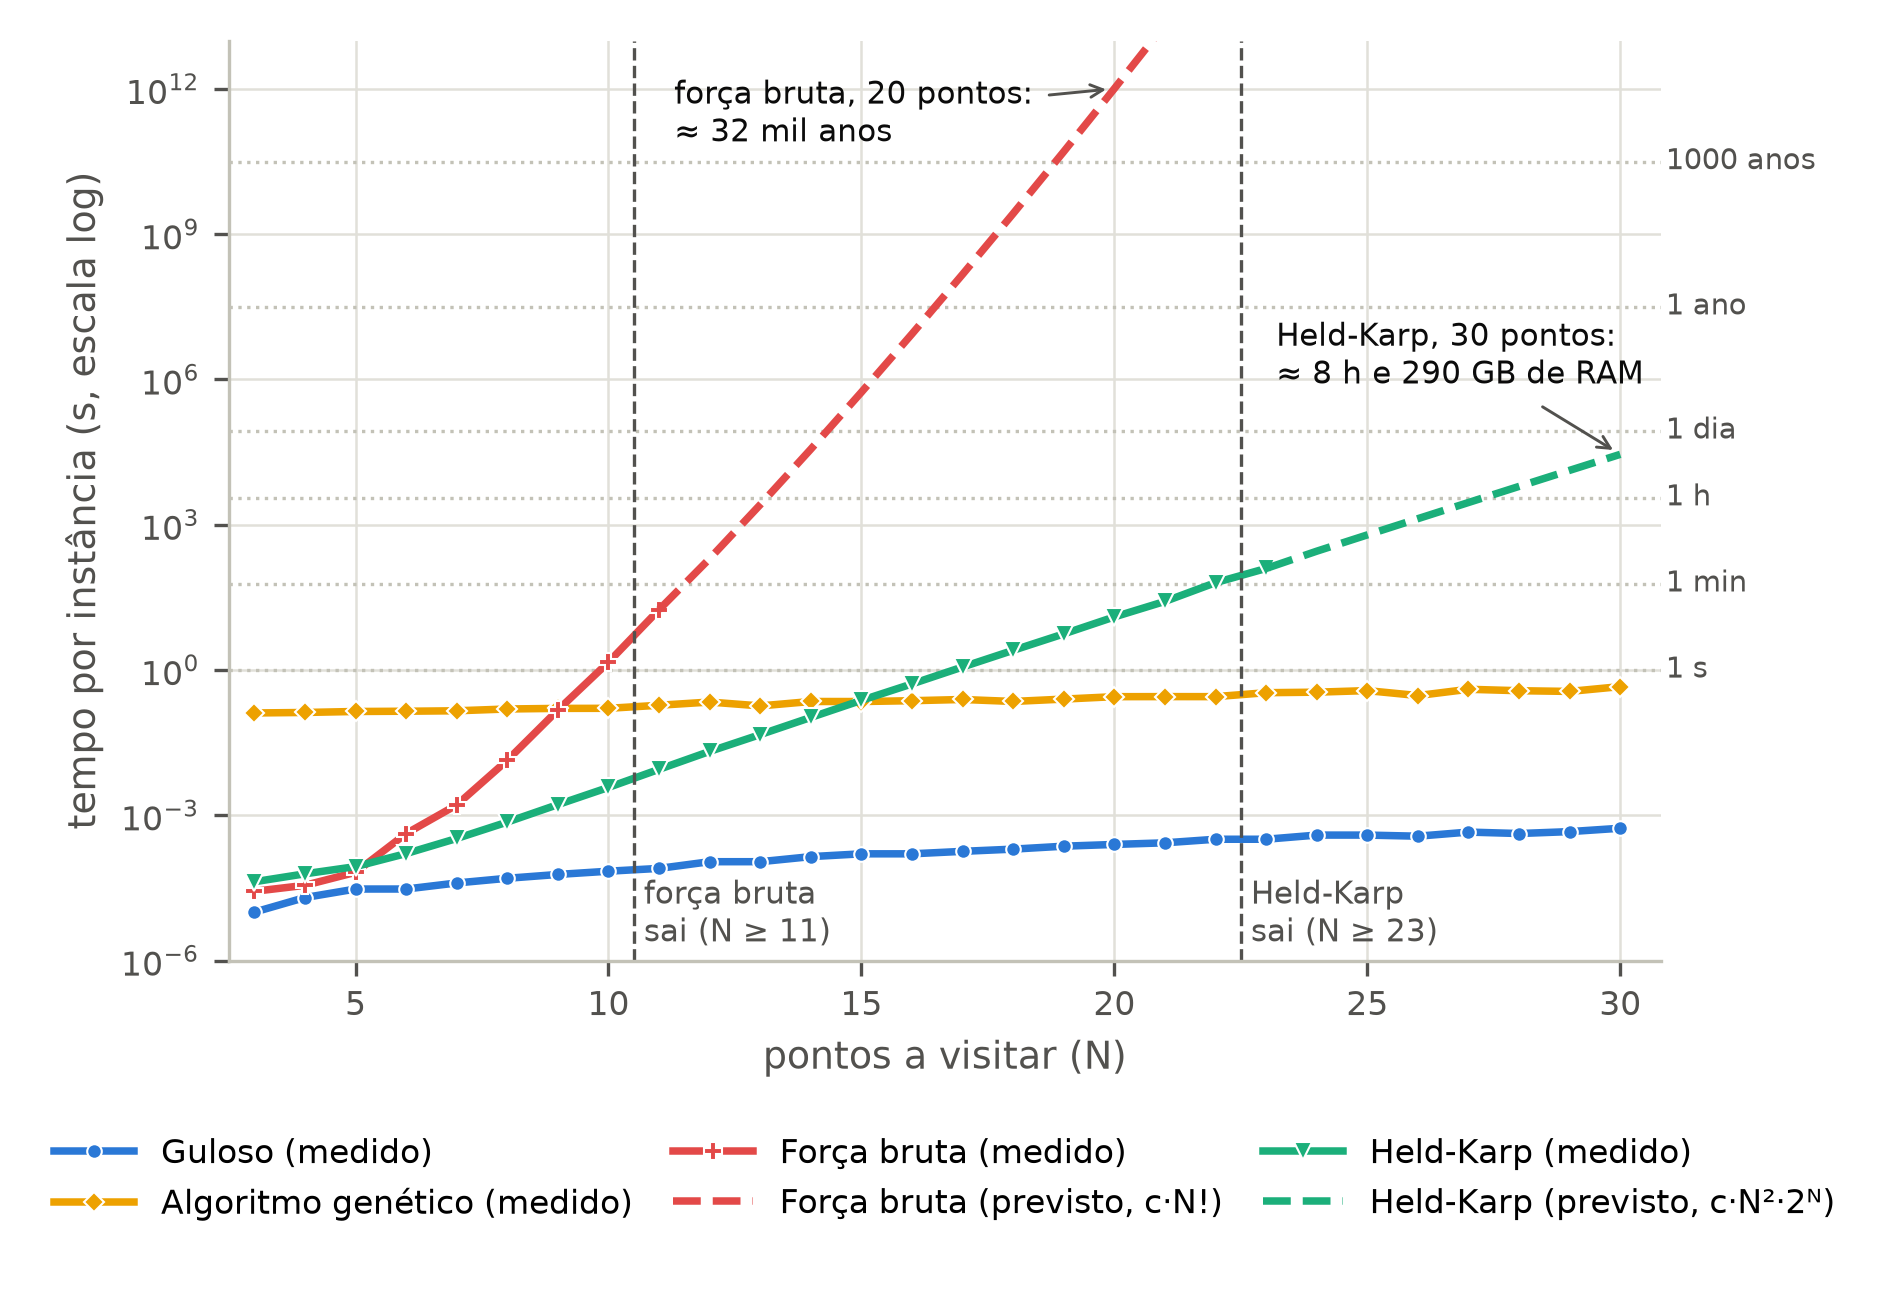
\includegraphics[width=\textwidth]{images/rotas/tempo_resolver.png}
    \fonte{elaborado pelos autores (2026).}
\end{figure}

\begin{figure}[H]
    \centering
    \caption{Memória necessária pelo Held-Karp e pelo algoritmo genético, por número de pontos.}
    \label{fig:rotas_memoria}
    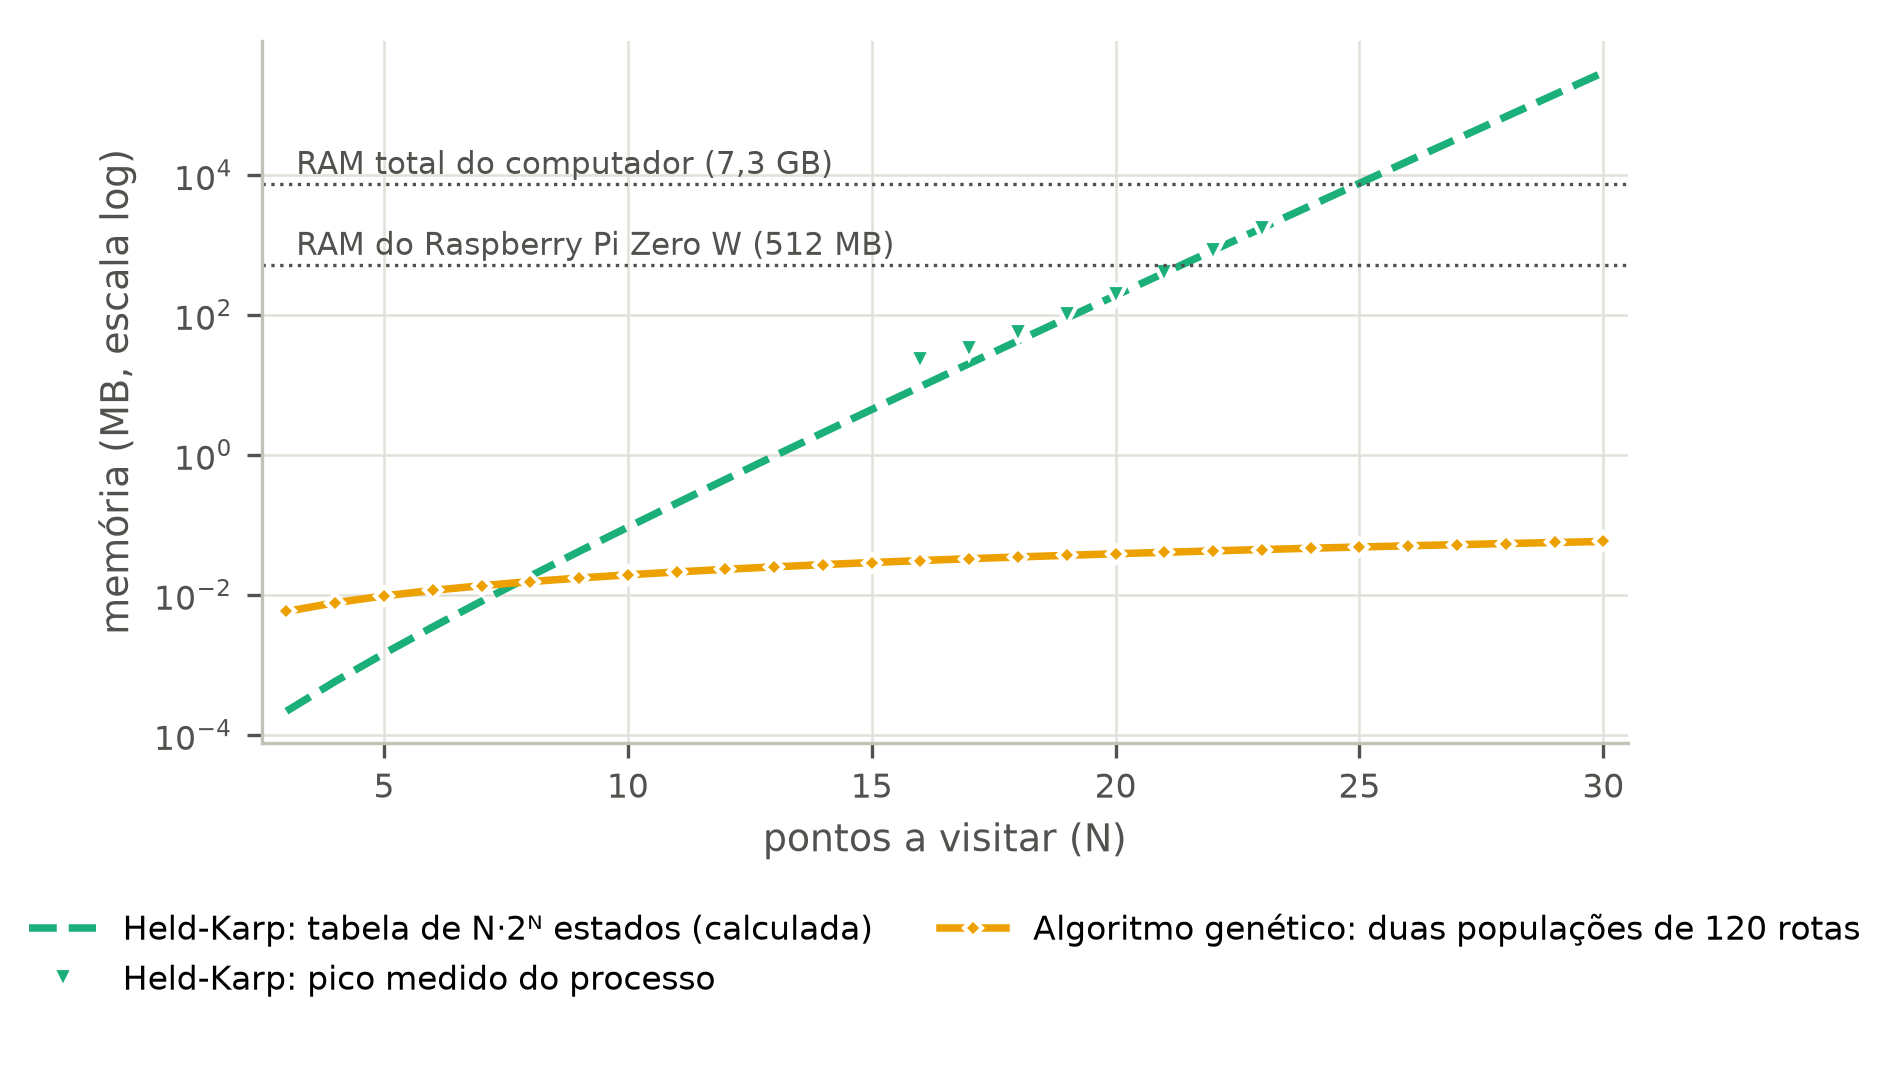
\includegraphics[width=\textwidth]{images/rotas/memoria_exato.png}
    \fonte{elaborado pelos autores (2026).}
\end{figure}

Com o critério da Seção~\ref{subsubsec:rotas_viabilidade}, cada método exato deixa o comparativo em um ponto diferente, o que divide os resultados em três faixas (Tabela~\ref{tab:rotas_fases}). Nas 80 instâncias em que os dois métodos exatos rodaram, os custos coincidiram em todas, o que confirma a implementação do Held-Karp.

\begin{table}[H]
    \centering
    \caption{Algoritmos executados em cada faixa de número de pontos.}
    \label{tab:rotas_fases}
    \small
    \renewcommand{\arraystretch}{1.25}
    \begin{tabular}{cccccc}
        \hline
        \textbf{Pontos ($N$)} & \textbf{Aleatório} & \textbf{Guloso} & \textbf{AG} & \textbf{Força bruta} & \textbf{Held-Karp} \\
        \hline
        3 a 10 & sim & sim & sim & sim & sim \\
        11 a 22 & sim & sim & sim & não & sim \\
        23 a 30 & sim & sim & sim & não & não \\
        \hline
    \end{tabular}
    \par\vspace{0.15cm}
    \footnotesize A força bruta sai com 11 pontos (18~s por instância e $\approx$ 3~min com 12); o Held-Karp sai com 23 (mais de 2~min e 1,7~GB) e não cabe na memória a partir de 25.\\
    Fonte: elaborado pelos autores (2026).
\end{table}

% ----------------------------------------------------------------
\subsection{Qualidade das rotas}\label{subsec:res_rotas_qualidade}
% ----------------------------------------------------------------

A Figura~\ref{fig:rotas_qualidade} apresenta a qualidade média das rotas, isto é, a razão entre o comprimento da rota de referência e o da rota obtida: 100\% corresponde à rota ótima (ou à melhor conhecida, acima de 22 pontos), e quanto maior o valor, melhor a rota. O AG manteve qualidade entre 96,5\% e 100\% em toda a faixa, o guloso entre 85\% e 94\%, e a ordem aleatória caiu de 74\% para 33\% com o aumento de $N$. As distâncias médias correspondentes estão na Tabela~\ref{tab:rotas_distancia}.

\begin{figure}[H]
    \centering
    \caption{Qualidade média das rotas, em relação à rota ótima ou à melhor conhecida (10 instâncias por $N$).}
    \label{fig:rotas_qualidade}
    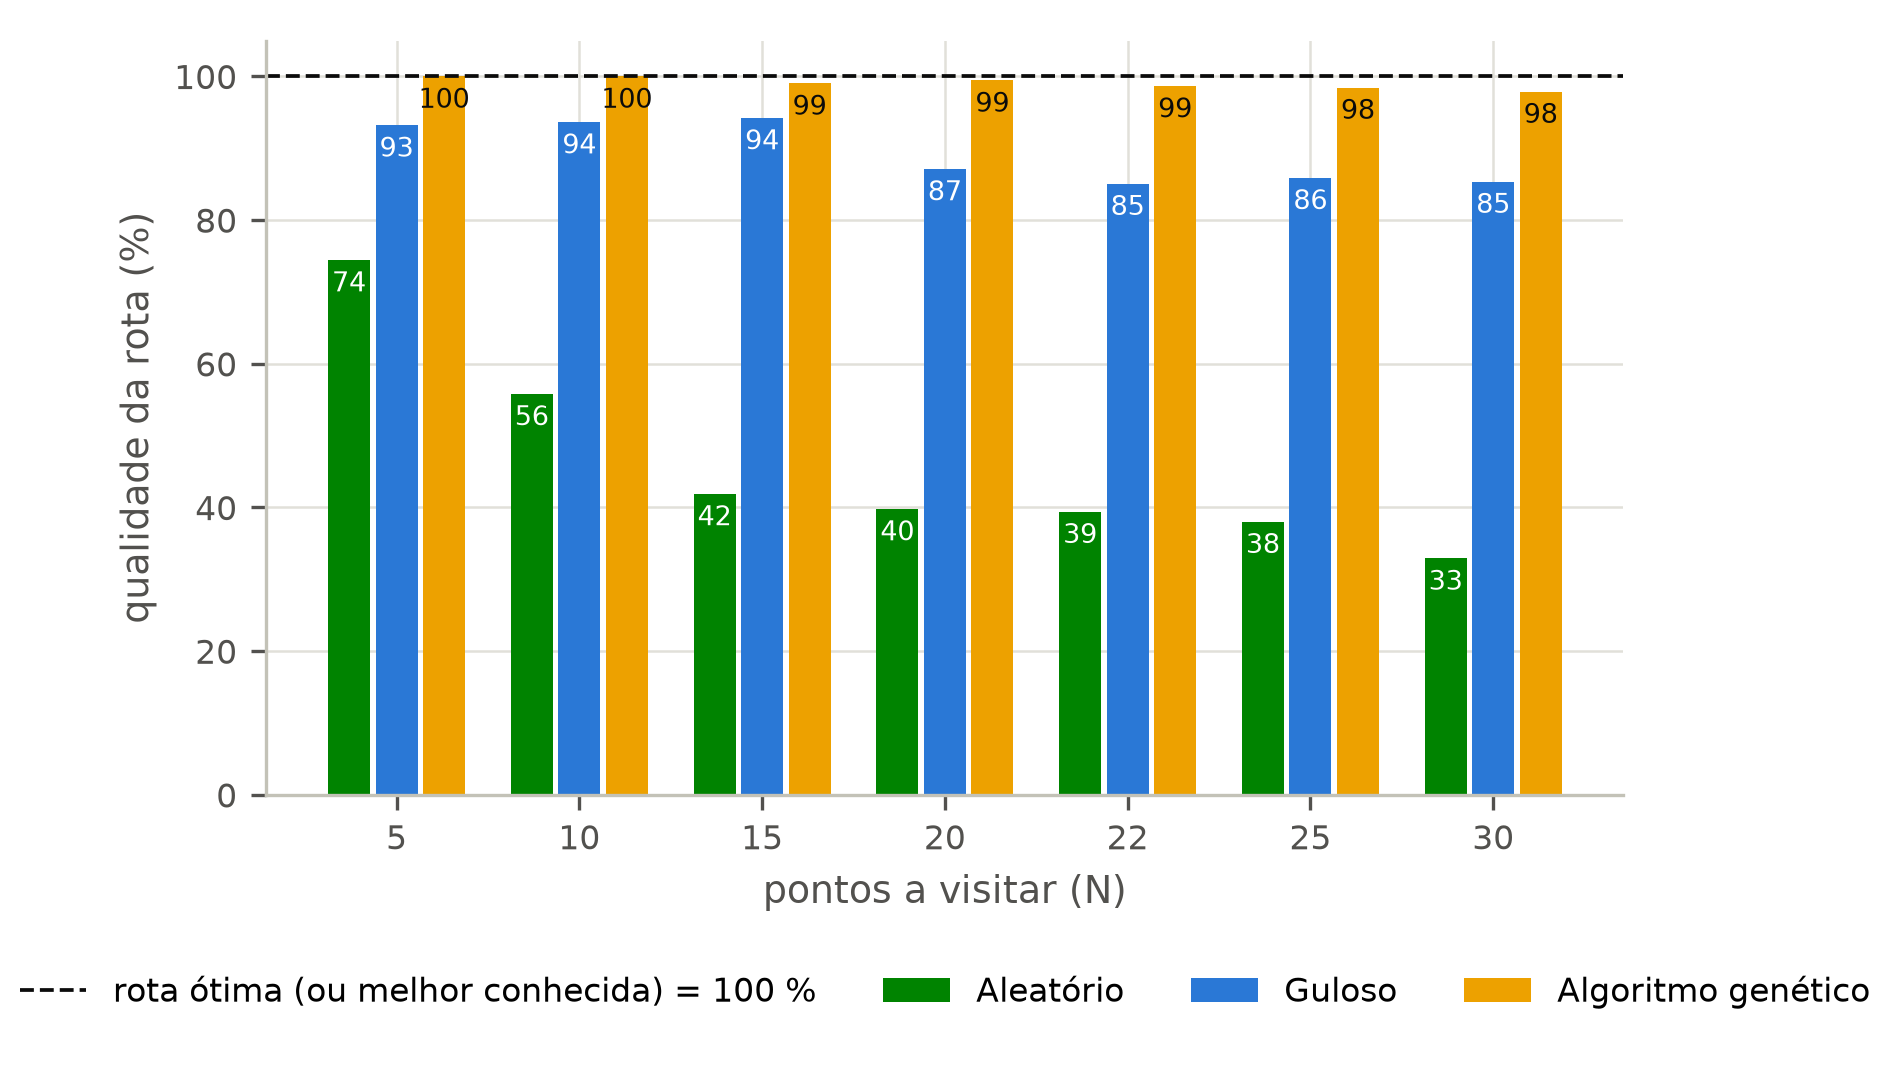
\includegraphics[width=\textwidth]{images/rotas/qualidade_rotas.png}
    \fonte{elaborado pelos autores (2026).}
\end{figure}

\begin{table}[H]
    \centering
    \caption{Distância média do circuito, em metros (10 instâncias por $N$).}
    \label{tab:rotas_distancia}
    \small
    \renewcommand{\arraystretch}{1.2}
    \begin{tabular}{cccccc}
        \hline
        \textbf{$N$} & \textbf{Aleatório} & \textbf{Guloso} & \textbf{AG} & \textbf{Força bruta} & \textbf{Held-Karp} \\
        \hline
        5 & 18,86 & 14,86 & 13,78 & 13,78 & 13,78 \\
        10 & 35,59 & 21,04 & 19,64 & 19,64 & 19,64 \\
        15 & 54,52 & 24,26 & 22,98 & --- & 22,76 \\
        20 & 65,12 & 29,82 & 25,94 & --- & 25,79 \\
        22 & 68,38 & 31,91 & 27,30 & --- & 26,93 \\
        25 & 77,76 & 34,34 & 29,76 & --- & --- \\
        30 & 98,44 & 38,04 & 32,96 & --- & --- \\
        \hline
    \end{tabular}
    \par\vspace{0.2cm}
    \footnotesize Fonte: elaborado pelos autores (2026).
\end{table}

A Tabela~\ref{tab:rotas_gap} agrupa o \textit{gap} e os acertos por faixa. Até 10 pontos, o AG obteve o ótimo global em todas as 80 instâncias; entre 11 e 22, em 70 de 120, com \textit{gap} médio de 0,85\%; entre 23 e 30, ficou em média 2,2\% acima da melhor rota conhecida. O guloso perdeu de 6,6\% a 18,3\% em média, chegando a 37\% em instâncias desfavoráveis.

\begin{table}[H]
    \centering
    \caption{\textit{Gap} médio, \textit{gap} máximo e acertos da referência, por faixa de $N$.}
    \label{tab:rotas_gap}
    \small
    \renewcommand{\arraystretch}{1.25}
    \setlength{\tabcolsep}{4pt}
    \begin{tabular}{lccc}
        \hline
        \textbf{Algoritmo} & \textbf{3 a 10 (ótimo)} & \textbf{11 a 22 (ótimo)} & \textbf{23 a 30 (melhor conhecida)} \\
        \hline
        Aleatório & 49,3\% (127,4\%) $\cdot$ 6/80 & 132,0\% (198,7\%) $\cdot$ 0/120 & 182,4\% (264,7\%) $\cdot$ 0/80 \\
        Guloso & 6,6\% (28,6\%) $\cdot$ 11/80 & 9,7\% (31,7\%) $\cdot$ 1/120 & 18,3\% (36,9\%) $\cdot$ 0/80 \\
        Algoritmo genético & 0,00\% (0,00\%) $\cdot$ 80/80 & 0,85\% (9,6\%) $\cdot$ 70/120 & 2,2\% (7,7\%) $\cdot$ 20/80 \\
        \hline
    \end{tabular}
    \par\vspace{0.15cm}
    \footnotesize Formato: \textit{gap} médio (\textit{gap} máximo) $\cdot$ instâncias em que a referência foi obtida.\\
    Fonte: elaborado pelos autores (2026).
\end{table}

A comparação instância a instância está na Tabela~\ref{tab:rotas_confronto}, em que cada célula indica em quantas das 280 instâncias o algoritmo da linha obteve rota mais curta que o da coluna. O AG superou o guloso em 262 instâncias e foi superado em 6; a ordem aleatória nunca superou o AG.

\begin{table}[H]
    \centering
    \caption{Instâncias, entre 280, em que o algoritmo da linha obteve rota mais curta que o da coluna.}
    \label{tab:rotas_confronto}
    \small
    \renewcommand{\arraystretch}{1.25}
    \begin{tabular}{lccc}
        \hline
        & \textbf{Aleatório} & \textbf{Guloso} & \textbf{AG} \\
        \hline
        \textbf{Aleatório} & --- & 9 & 0 \\
        \textbf{Guloso} & 270 & --- & 6 \\
        \textbf{AG} & 274 & 262 & --- \\
        \hline
    \end{tabular}
    \par\vspace{0.15cm}
    \footnotesize Empates (rotas de mesmo comprimento): aleatório e guloso, 1; aleatório e AG, 6; guloso e AG, 12.\\
    Fonte: elaborado pelos autores (2026).
\end{table}

As Figuras~\ref{fig:rotas_3d_n10} a \ref{fig:rotas_3d_n25} mostram as rotas em 3D de três instâncias. Com 10 e 20 pontos, o Held-Karp fornece o ótimo global, e o AG obtém exatamente a mesma rota, enquanto o guloso fica 26,1\% e 30,7\% acima, respectivamente. Com 25 pontos, o Held-Karp não pode ser executado, e o ótimo global é desconhecido. É nesse cenário que o \textit{benchmark} se mostra necessário: como o AG obteve o ótimo ou ficou próximo dele em todas as faixas em que o ótimo era conhecido, sua rota de 30,35~m é adotada como solução de referência prática, contra 34,14~m do guloso e 89,61~m da ordem aleatória.

\begin{figure}[H]
    \centering
    \caption{Rotas de 10 pontos obtidas pelos quatro algoritmos.}
    \label{fig:rotas_3d_n10}
    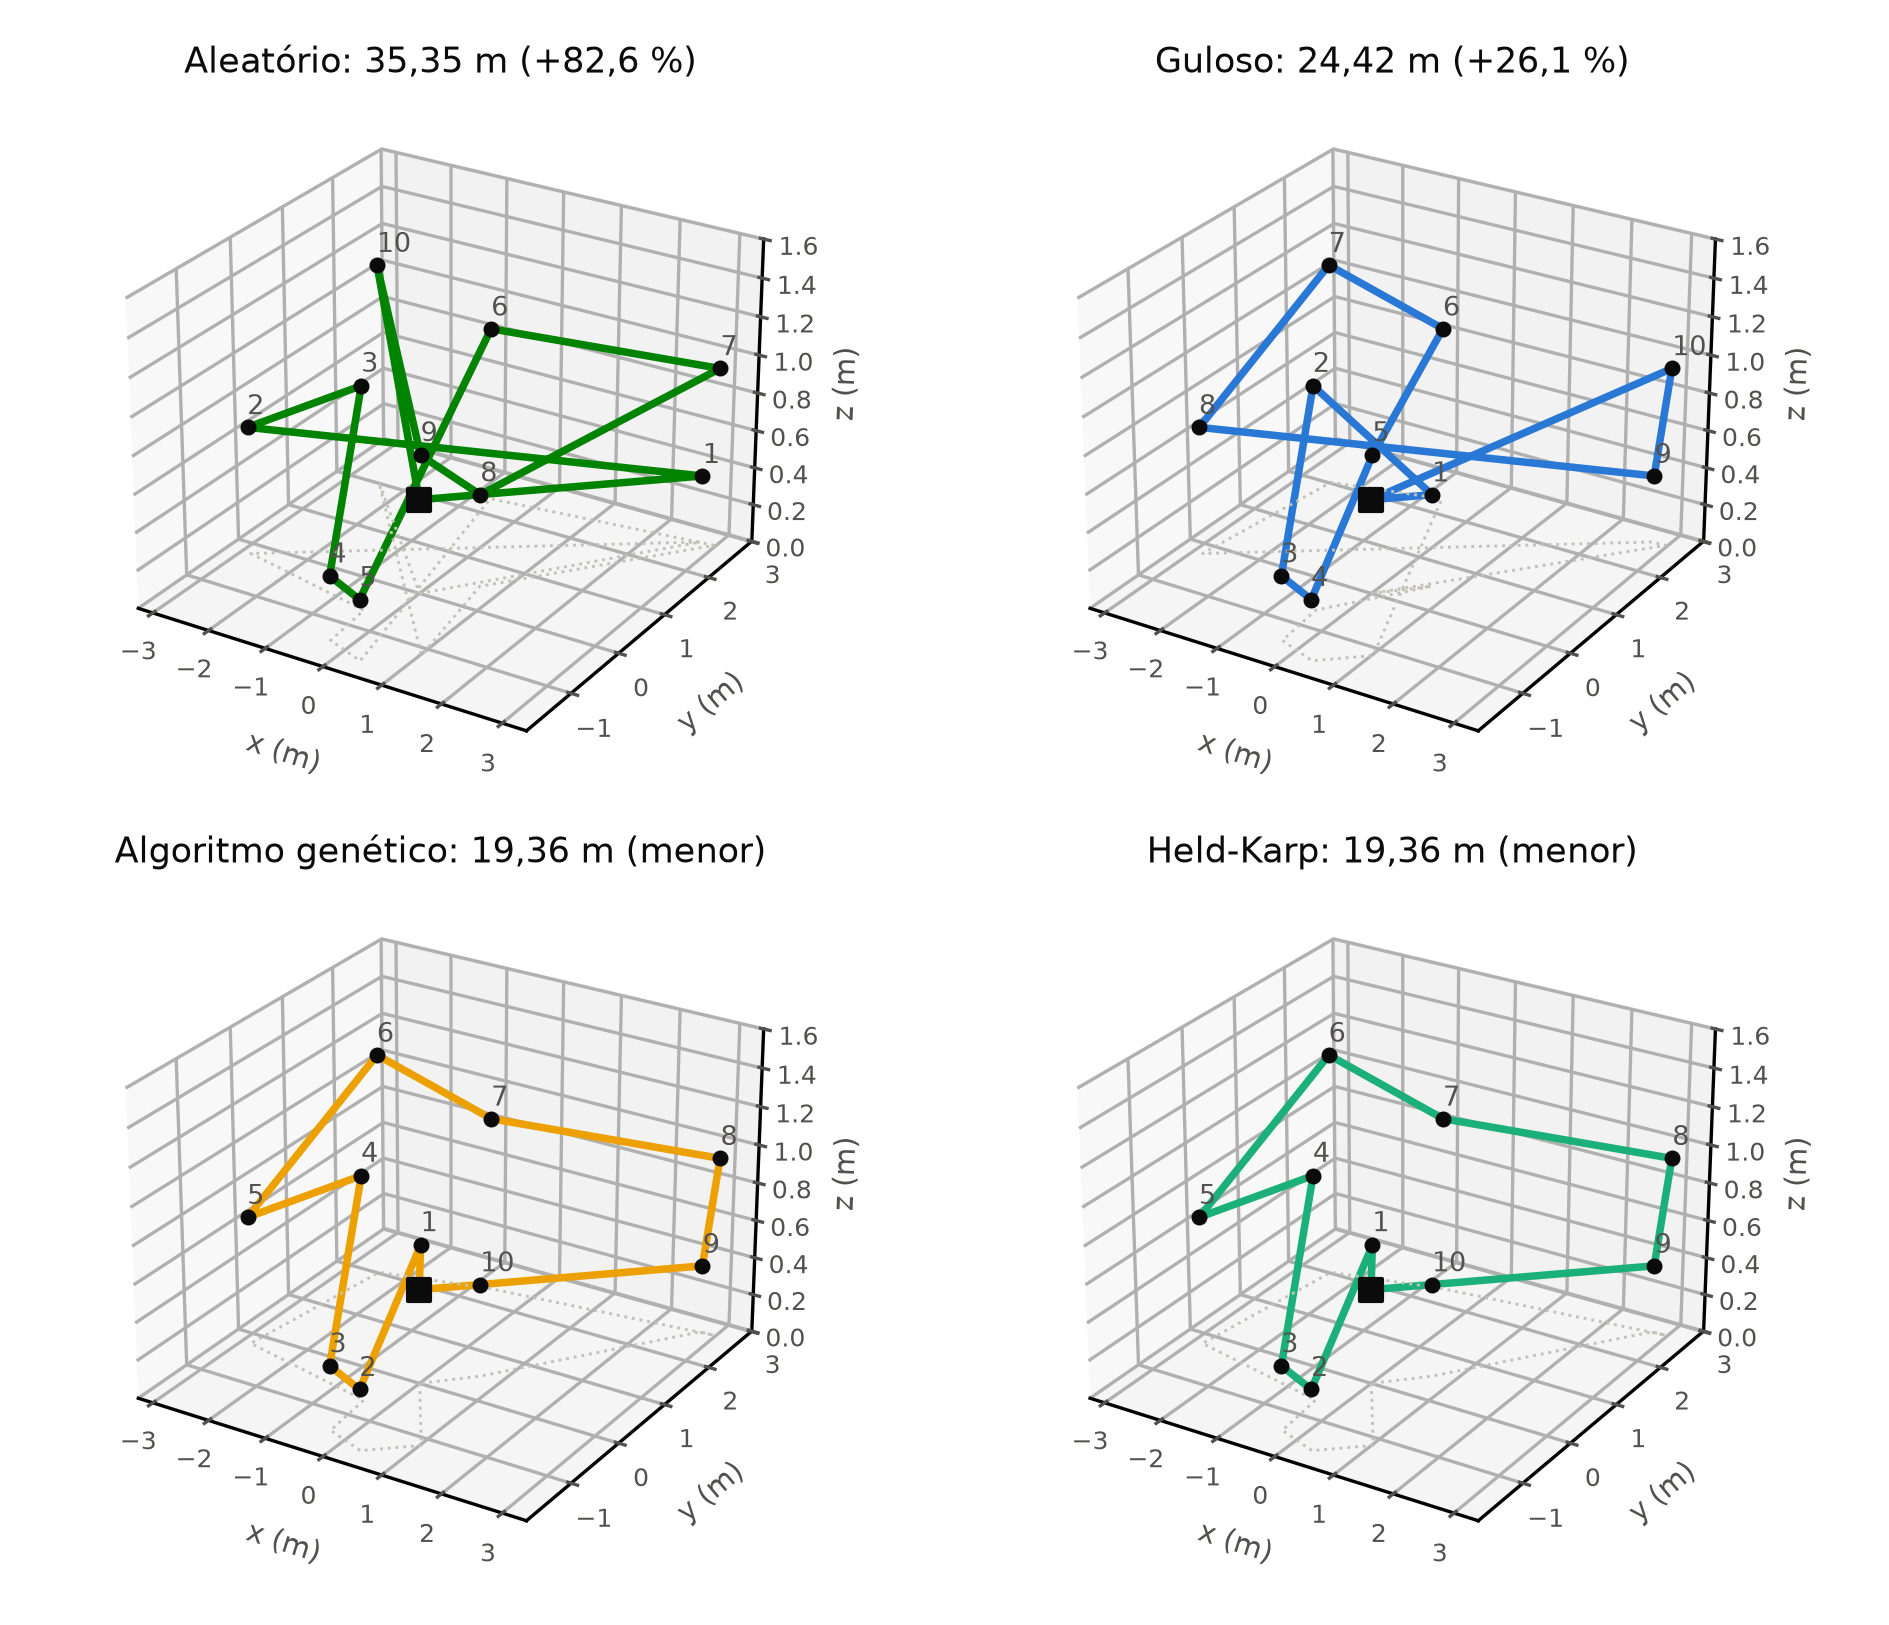
\includegraphics[width=\textwidth]{images/rotas/rotas_3d_n10.png}
    \fonte{elaborado pelos autores (2026).}
\end{figure}

\begin{figure}[H]
    \centering
    \caption{Rotas de 20 pontos obtidas pelos quatro algoritmos.}
    \label{fig:rotas_3d_n20}
    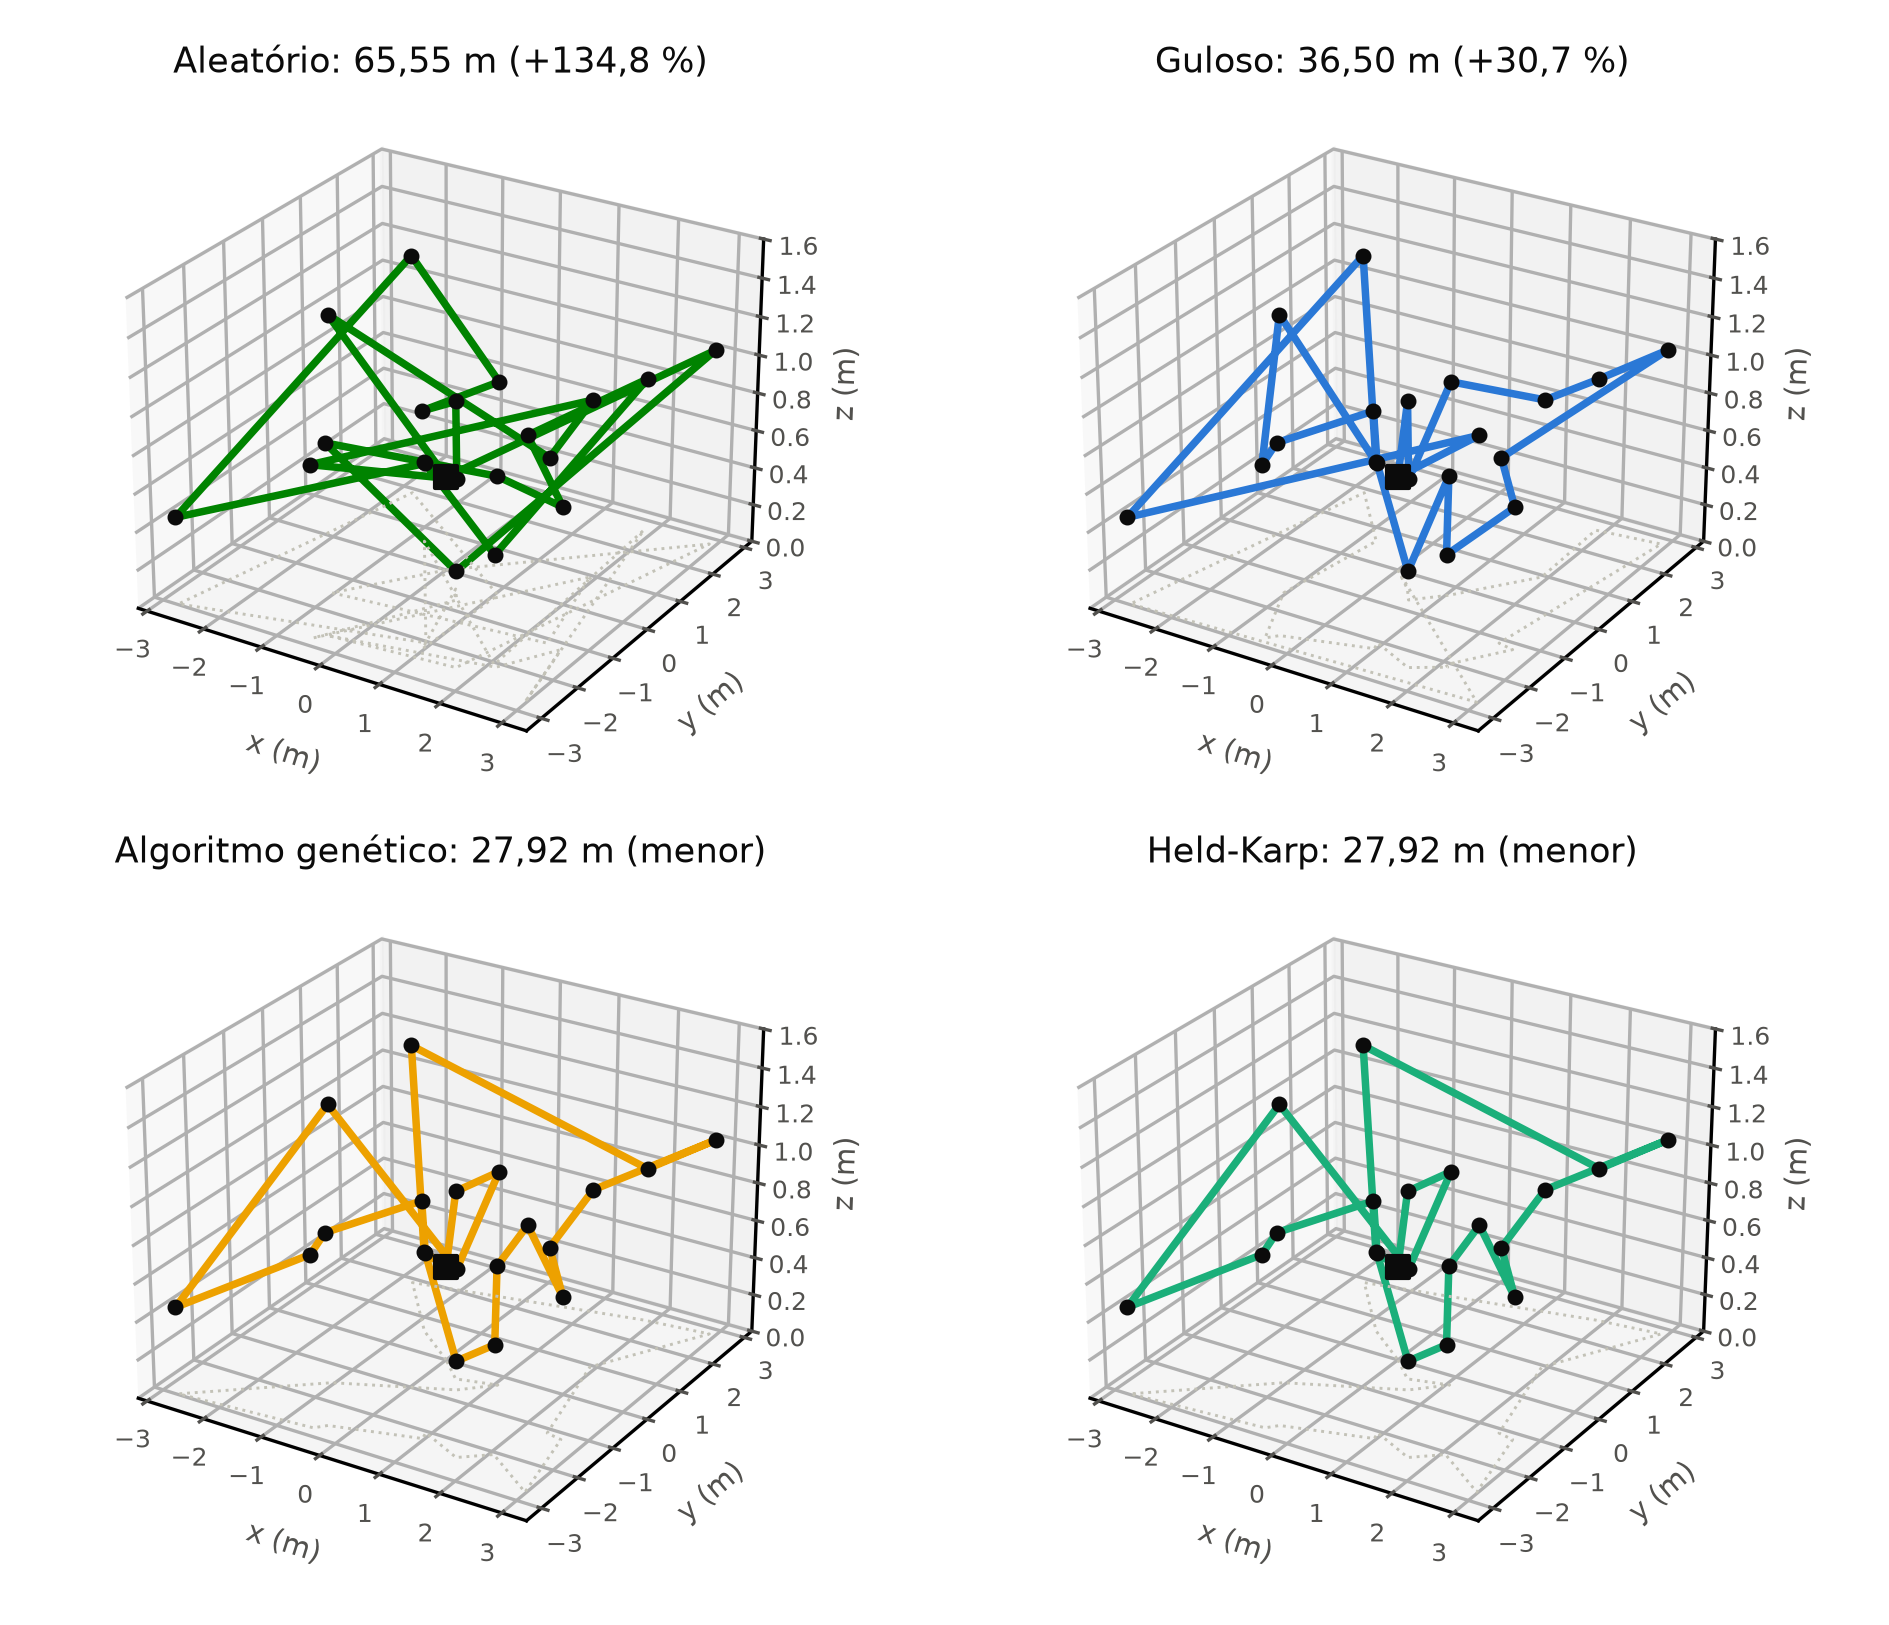
\includegraphics[width=\textwidth]{images/rotas/rotas_3d_n20.png}
    \fonte{elaborado pelos autores (2026).}
\end{figure}

\begin{figure}[H]
    \centering
    \caption{Rotas de 25 pontos, em que o Held-Karp não cabe na memória do computador.}
    \label{fig:rotas_3d_n25}
    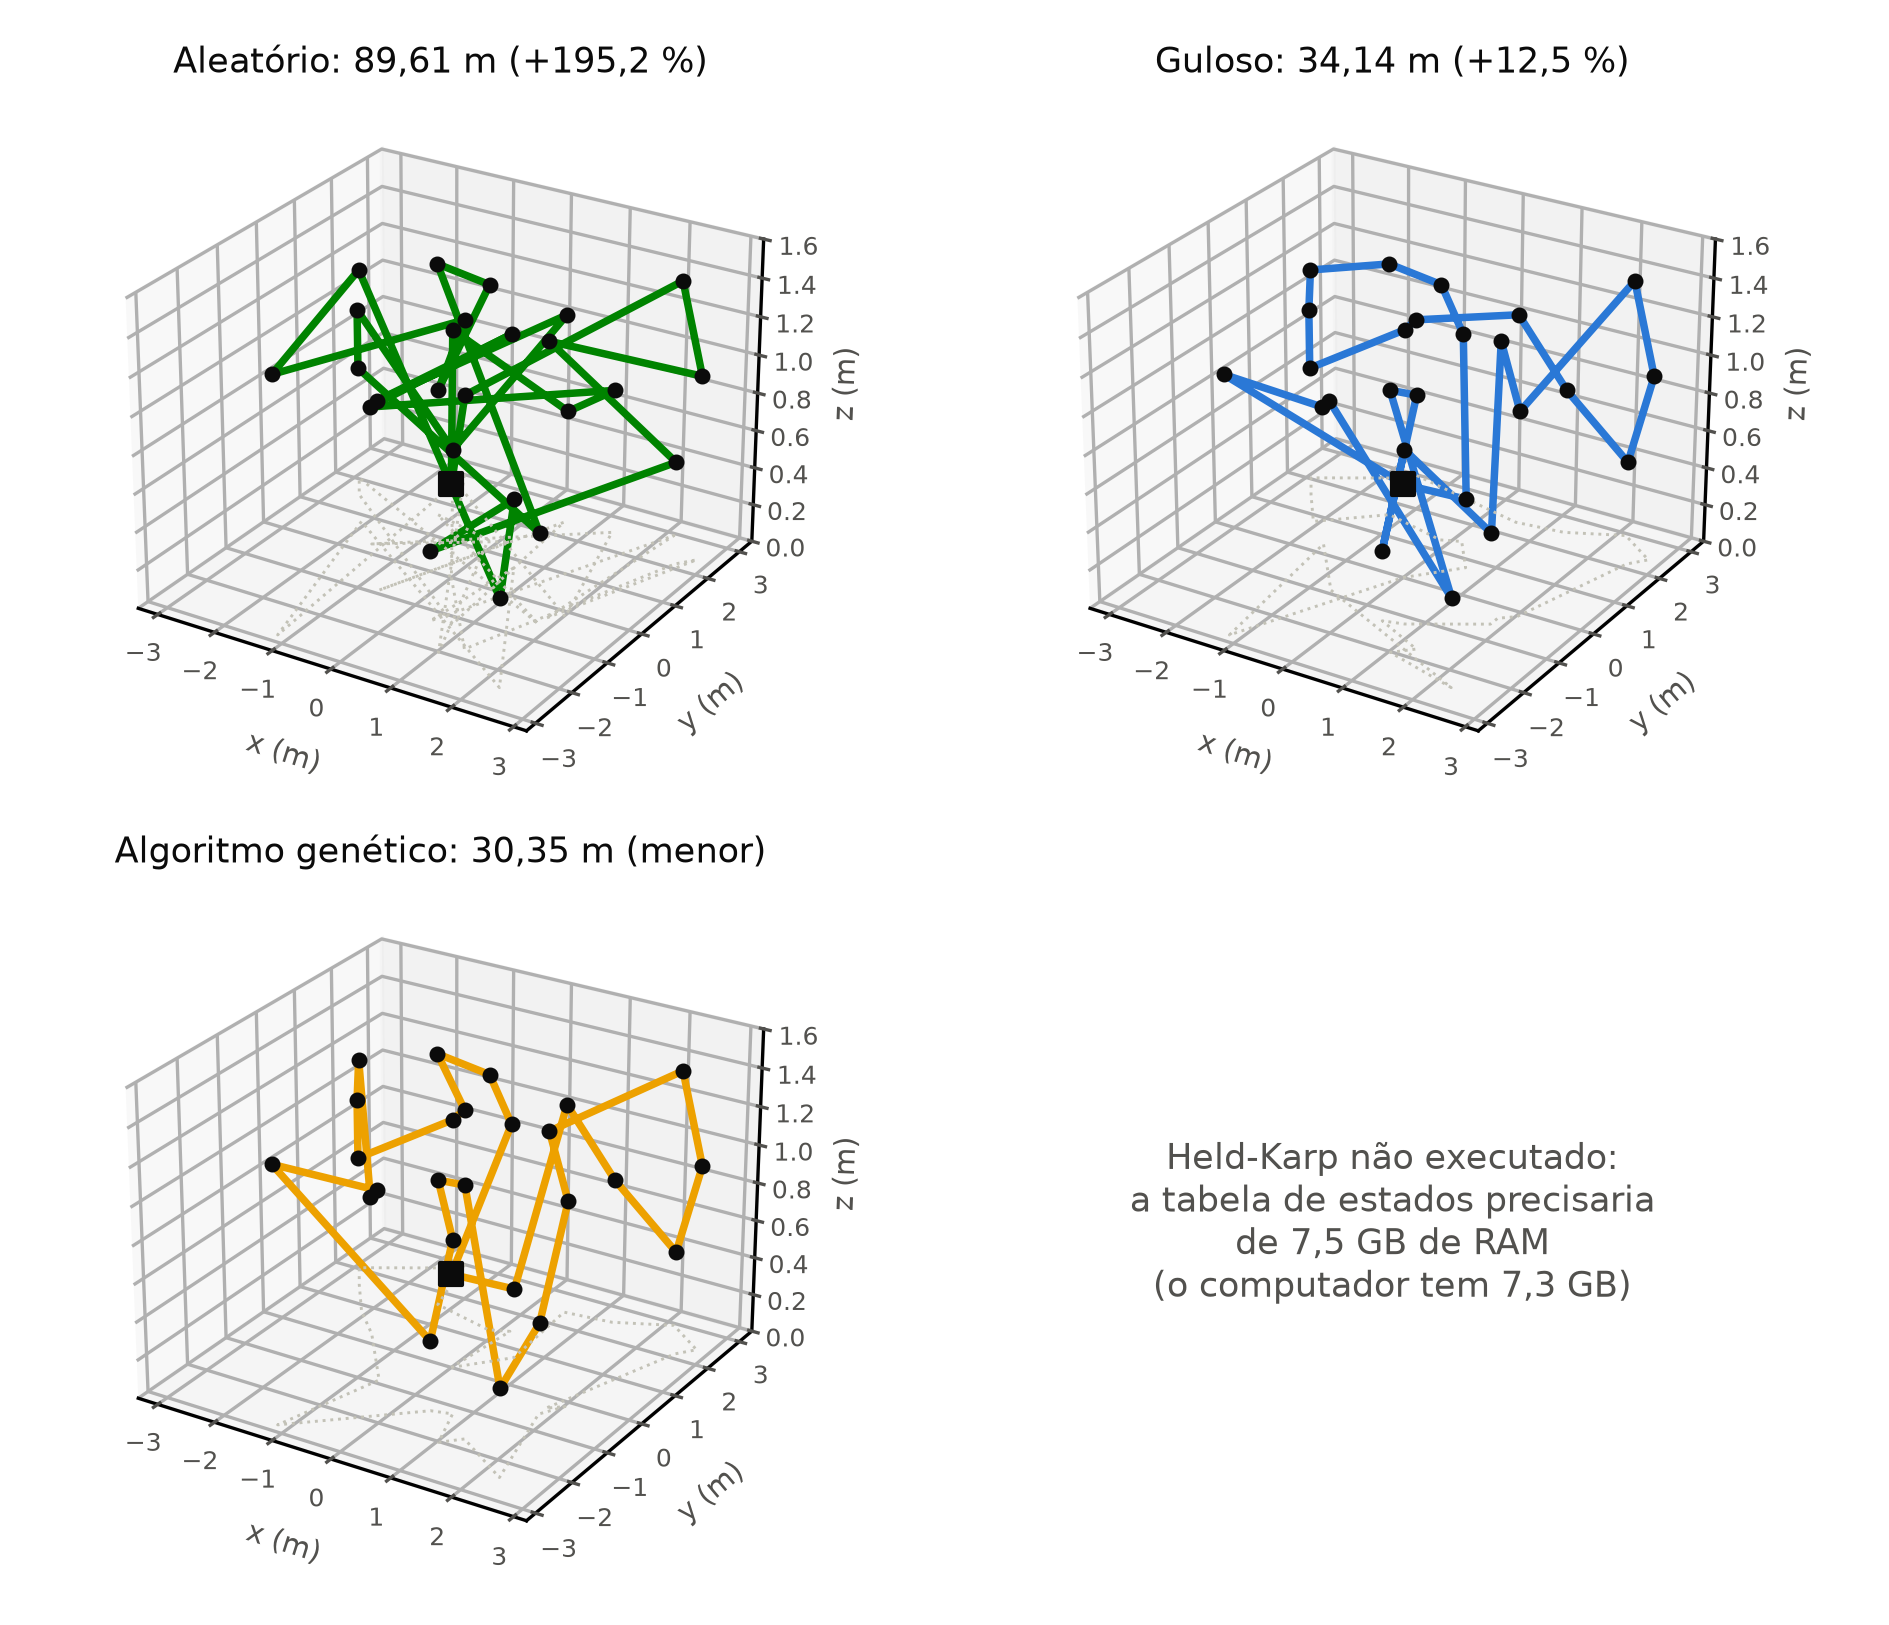
\includegraphics[width=\textwidth]{images/rotas/rotas_3d_n25.png}
    \fonte{elaborado pelos autores (2026).}
\end{figure}

% ----------------------------------------------------------------
\subsection{Tempo de cálculo}\label{subsec:res_rotas_tempo}
% ----------------------------------------------------------------

A Tabela~\ref{tab:rotas_tempo} apresenta o tempo médio de cálculo por instância no \textit{benchmark}. O AG levou de 0,13 a 0,45~s em toda a faixa, valor dominado pelo número de gerações (média de 272, mínimo de 200 e máximo de 665) e pouco sensível a $N$. A força bruta já é mais lenta que o AG com 10 pontos, e o Held-Karp, a partir de 15. Os tempos variaram cerca de 10\% entre execuções repetidas, conforme a carga do computador; as rotas e distâncias não se alteraram.

\begin{table}[H]
    \centering
    \caption{Tempo médio de cálculo por instância.}
    \label{tab:rotas_tempo}
    \small
    \renewcommand{\arraystretch}{1.2}
    \begin{tabular}{ccccc}
        \hline
        \textbf{$N$} & \textbf{Guloso} & \textbf{AG} & \textbf{Força bruta} & \textbf{Held-Karp} \\
        \hline
        5 & 0,03~ms & 139~ms & 0,06~ms & 0,07~ms \\
        10 & 0,07~ms & 162~ms & 1,56~s & 4,1~ms \\
        15 & 0,16~ms & 223~ms & --- & 260~ms \\
        20 & 0,25~ms & 281~ms & --- & 13,0~s \\
        22 & 0,32~ms & 282~ms & --- & 63,7~s \\
        25 & 0,39~ms & 376~ms & --- & --- \\
        30 & 0,54~ms & 454~ms & --- & --- \\
        \hline
    \end{tabular}
    \par\vspace{0.2cm}
    \footnotesize Fonte: elaborado pelos autores (2026).
\end{table}

% ----------------------------------------------------------------
\subsection{Convergência do algoritmo genético}\label{subsec:res_rotas_convergencia}
% ----------------------------------------------------------------

A Figura~\ref{fig:rotas_convergencia} mostra a evolução do melhor indivíduo do AG na primeira instância de quatro valores de $N$. A população inicial, aleatória, começa entre 35\% e 150\% acima da referência e melhora rapidamente nas primeiras 50 a 150 gerações, superando o guloso. Depois, a melhora cessa: com 10 e 20 pontos o AG atingiu o ótimo global, mas com 15 pontos estabilizou 3,4\% acima dele (24,27~m contra 23,47~m), preso em um ótimo local, isto é, uma rota que as operações do AG não conseguiram mais encurtar, embora existisse uma rota menor.

\begin{figure}[H]
    \centering
    \caption{Convergência do melhor indivíduo do algoritmo genético.}
    \label{fig:rotas_convergencia}
    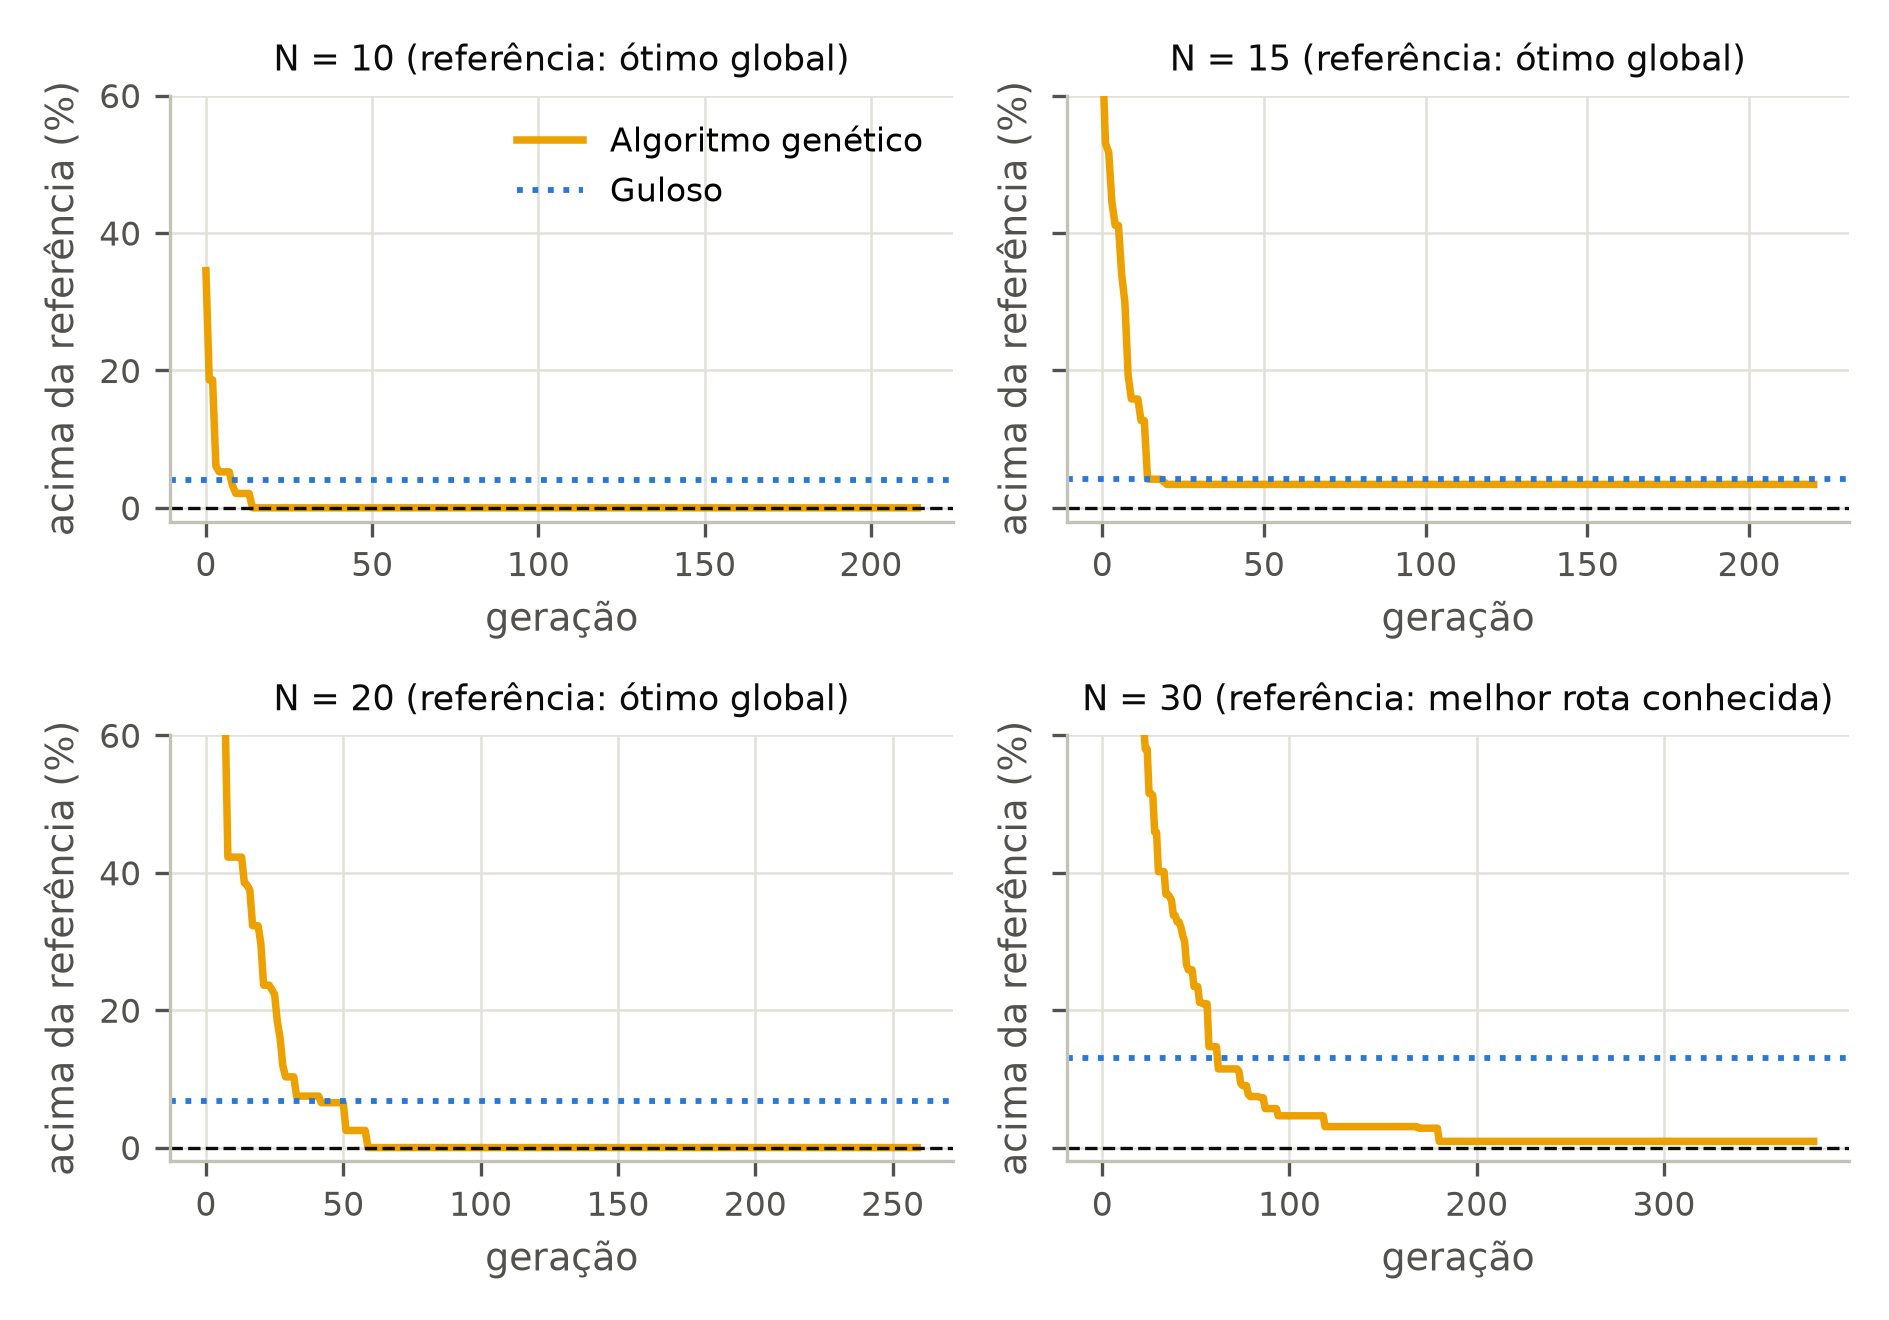
\includegraphics[width=\textwidth]{images/rotas/convergencia_genetico.png}
    \fonte{elaborado pelos autores (2026).}
\end{figure}

% ----------------------------------------------------------------
\subsection{Investigação complementar: busca local 2-opt}\label{subsec:res_rotas_2opt}
% ----------------------------------------------------------------

Durante o desenvolvimento, identificou-se na literatura que a busca local repetida a partir de várias rotas iniciais é uma alternativa competitiva para o TSP \cite{johnson1997}. Por isso, a busca local 2-opt com 20 partidas aleatórias foi incluída no \textit{benchmark} de forma exploratória, sem estudo aprofundado de seus parâmetros. A Tabela~\ref{tab:rotas_2opt} compara seus resultados com os do AG.

\begin{table}[H]
    \centering
    \caption{Comparação exploratória entre o AG e a busca local 2-opt com 20 partidas.}
    \label{tab:rotas_2opt}
    \small
    \renewcommand{\arraystretch}{1.25}
    \begin{tabular}{lcc}
        \hline
        \textbf{Indicador} & \textbf{AG} & \textbf{2-opt com 20 partidas} \\
        \hline
        Ótimo global obtido (instâncias de até 22 pontos) & 150 de 200 & 189 de 200 \\
        \textit{Gap} médio entre 11 e 22 pontos & 0,85\% & 0,04\% \\
        \textit{Gap} médio entre 23 e 30 pontos & 2,2\% & 0,05\% \\
        Tempo médio com 30 pontos & 454~ms & 16~ms \\
        Rota mais curta que a do outro (280 instâncias) & 8 & 106 \\
        \hline
    \end{tabular}
    \par\vspace{0.15cm}
    \footnotesize As 166 instâncias restantes terminaram empatadas.\\
    Fonte: elaborado pelos autores (2026).
\end{table}

Nos dados obtidos, a busca local com múltiplas partidas foi superior ao AG em qualidade e cerca de 30 vezes mais rápida. A análise das partidas ajuda a explicar o resultado: com 30 pontos, as 20 partidas convergiram em média para 18 ótimos locais diferentes, e somente 5,5\% delas alcançaram a melhor rota. Uma única busca local, portanto, fica facilmente presa em um ótimo local, mas repeti-la a partir de pontos de partida diferentes aumenta muito a chance de alcançar o ótimo global. Verificou-se também que 277 das 280 rotas do AG já eram ótimos locais em relação ao 2-opt; ou seja, o AG encontra ótimos locais com frequência, mas nem sempre o global. Como essa abordagem não foi estudada em profundidade, ela é indicada como alternativa a ser explorada em trabalhos futuros.

% ----------------------------------------------------------------
\subsection{Execução das rotas no controlador de voo}\label{subsec:res_rotas_stm32}
% ----------------------------------------------------------------

As rotas de uma instância tridimensional de 6 pontos, com alturas de 64 a 145~cm, foram executadas pelo STM32 com o VANT simulado, conforme a Seção~\ref{subsubsec:rotas_execucao_stm32} (Tabela~\ref{tab:rotas_stm32}). O AG obteve a mesma rota do Held-Karp percorrida no sentido inverso, com o mesmo comprimento, 21,3\% menor que a do guloso. Em todas as execuções, o VANT simulado chegou a cada ponto com erro máximo de 3,1~cm, dentro da tolerância de 5~cm usada pelo STM32 para declarar estabilidade.

\begin{table}[H]
    \centering
    \caption{Rotas tridimensionais executadas pelo STM32 com o VANT simulado.}
    \label{tab:rotas_stm32}
    \small
    \renewcommand{\arraystretch}{1.2}
    \begin{tabular}{ccccc}
        \hline
        \textbf{Algoritmo} & \textbf{Ordem} & \textbf{Circuito 3D} & \textbf{Trechos executados} & \textbf{Maior erro em um ponto} \\
        \hline
        Guloso & 3 4 5 2 1 6 & 1898~cm & 14 & 3,0~cm \\
        AG & 3 4 6 5 2 1 & 1493~cm ($-21{,}3\%$) & 14 & 3,0~cm \\
        Held-Karp & 1 2 5 6 4 3 & 1493~cm ($-21{,}3\%$) & 14 & 3,1~cm \\
        \hline
    \end{tabular}
    \par\vspace{0.15cm}
    \footnotesize Pontos (cm): $(-177, 188, 129)$, $(-104, -150, 145)$, $(43, -43, 99)$, $(62, -71, 64)$, $(92, -204, 93)$ e $(298, -274, 134)$.\\
    Fonte: elaborado pelos autores (2026).
\end{table}

% ----------------------------------------------------------------
\subsection{Execução do algoritmo genético no Raspberry Pi Zero W}\label{subsec:res_rotas_pi}
% ----------------------------------------------------------------

A Tabela~\ref{tab:rotas_pi} compara a rota obtida pelo AG no computador pessoal e no Raspberry Pi Zero W para três instâncias: o quadrado de 40~cm executado com o VANT simulado no STM32 no ensaio de comunicação (Seção~\ref{subsec:res_com_missao}) e duas instâncias do \textit{benchmark}, com 10 e 30 pontos. Nas três, a ordem, o comprimento e a assinatura SHA-256 foram idênticos nas duas máquinas: o Raspberry Pi calcula exatamente a mesma rota, e os resultados de qualidade do \textit{benchmark} valem para o algoritmo embarcado. Os 26 testes automatizados do programa também foram aprovados no próprio Raspberry Pi.

\begin{table}[H]
    \centering
    \caption{Mesma rota calculada pelo AG no computador pessoal e no Raspberry Pi Zero W.}
    \label{tab:rotas_pi}
    \small
    \renewcommand{\arraystretch}{1.2}
    \begin{tabular}{lccccc}
        \hline
        \textbf{Instância} & \textbf{Comprimento} & \textbf{SHA-256} & \textbf{PC} & \textbf{Raspberry Pi} & \textbf{Razão} \\
        \hline
        Quadrado de 40~cm & 160,0~cm & \texttt{52d2b0c4\ldots} & 0,14~s & 9,70~s & 69$\times$ \\
        10 pontos & 19,36~m & \texttt{9ffc5830\ldots} & 0,16~s & 11,14~s & 70$\times$ \\
        30 pontos & 30,84~m & \texttt{11f260a1\ldots} & 0,39~s & 23,92~s & 61$\times$ \\
        \hline
    \end{tabular}
    \par\vspace{0.15cm}
    \footnotesize A assinatura é a mesma nas duas máquinas; são mostrados os 8 primeiros dígitos hexadecimais. Tempos de uma execução de cada instância.\\
    Fonte: elaborado pelos autores (2026).
\end{table}

O Raspberry Pi foi de 61 a 70 vezes mais lento, levando de 10 a 24~s para ordenar de 3 a 30 pontos. Como a ordem é calculada uma única vez, antes da execução da rota, e cada trecho leva vários segundos para ser voado, esse tempo é aceitável para a aplicação. Os métodos exatos, por outro lado, seriam ainda mais limitados na placa: além de dezenas de vezes mais lentos, o Held-Karp ultrapassa metade dos 512~MB de RAM a partir de 21 pontos (Seção~\ref{subsec:res_rotas_limite}).

% ----------------------------------------------------------------
\subsection{Discussão}\label{subsec:res_rotas_discussao}
% ----------------------------------------------------------------

Os resultados confirmam que a obtenção do ótimo global se torna inviável com poucas dezenas de pontos, mesmo com o melhor dos métodos exatos avaliados. A força bruta, que traduz diretamente a definição do problema, deixa de ser praticável com 11 pontos. O Held-Karp estende esse limite para 22 pontos, sendo cerca de $10^{11}$ vezes mais rápido que a força bruta com 20 pontos, ao custo de uma tabela de estados que dobra a cada ponto adicionado; com 25 pontos, a memória necessária excede a do computador utilizado e, no Raspberry Pi Zero W, o limite é ainda menor.

O algoritmo genético manteve tempo inferior a 0,5~s e memória inferior a 0,1~MB em toda a faixa, com rotas iguais ao ótimo até 10 pontos e, em média, até 3,7\% acima da referência nas faixas maiores. Isso o torna viável exatamente onde os métodos exatos deixam de ser, e o \textit{benchmark} nas faixas em que o ótimo é conhecido fundamenta o uso de sua rota quando o ótimo não pode ser calculado. O guloso, embora mais rápido, perdeu de 6\% a 18\% de distância em média, e a ordem aleatória chegou a três vezes o comprimento ótimo.

No Raspberry Pi Zero W, o mesmo AG produziu exatamente as mesmas rotas, com tempo de 10 a 24~s, de 60 a 70 vezes maior que no computador pessoal. Esses resultados sustentam a viabilidade do algoritmo genético como solução adotada e validada no projeto, com qualidade de rota e tempo de cálculo compatíveis com o planejamento antes do voo. A validação de sua execução no Raspberry Pi e da integração com o controlador de voo fundamenta sua utilização no protótipo, mas não demonstra superioridade em relação a todas as alternativas avaliadas.

Um limite deve ser considerado: o AG implementado não usa busca local, ou seja, não tenta encurtar as rotas por pequenas modificações sistemáticas, e pode estabilizar em um ótimo local, como observado com 15 pontos. A investigação complementar indicou que a busca local repetida obteve rotas melhores em menos tempo; combiná-la ao AG, formando um algoritmo memético \cite{moscato1989}, ou adotá-la diretamente são caminhos para trabalhos futuros.

